\documentclass[acmlarge]{acmart}



\AtBeginDocument{%
  \providecommand\BibTeX{{%
    Bib\TeX}}}
  \settopmatter{printacmref=false}

\renewcommand{\descriptionlabel}[1]{\hspace{\labelsep}\textit{#1}}
\usepackage{xcolor}
\usepackage{multicol}
\usepackage{geometry}
\newcommand{\todo}{{\color{red}\textbf{TODO} }}
\newcommand{\disease}{{\small \texttt{DISEASE}} }
\newcommand{\hospital}{{\small \texttt{HOSPITAL}} }
\newcommand{\storage}{{\small \texttt{STORAGE}} }

% christos 1, 4
% vasilis 2, 3

\usepackage{amsmath}
\usepackage{subfig}

\usepackage{hyperref}
\usepackage{algorithm}
\usepackage{algpseudocodex}
\newcommand{\algorithmautorefname}{Algorithm}

\begin{document}

\title{The Map-Reduce Programming Paradigm}
\subtitle{M.Sc. course on ``Technologies for Big Data Analysis'' - Assignment 2}

\author{Christos Balaktsis (506)}
\email{balaktsis@csd.auth.gr}
\author{Vasileios Papastergios (505)}
\email{papster@csd.auth.gr}
\affiliation{
  \institution{Aristotle University}
  \city{Thessaloniki}
  \country{Greece}
}

\renewcommand{\shortauthors}{C. Balaktsis and V. Papastergios}
\maketitle

\section{Introduction}

The current document is a technical report for the second programming assignment in the M.Sc. course on
\emph{Technologies for Big Data Analysis}, offered by the \emph{DWS M.Sc Program}\footnote{https://dws.csd.auth.gr/} of the Aristotle University of Thessaloniki, Greece. The course is taught by Professor Apostolos Papadopoulos~\footnote{https://datalab-old.csd.auth.gr/$\sim$apostol/}. The authors attended the course during their first year of Ph.D. studies at the Institution.

The assignment contains 4 sub-problems and is part of a series, comprising 3 programming assignments on the following topics:
\begin{description}
  \item[Assignment 1] Multi-threading Programming and Inter-Process Communication
  \item[Assignment 2] The Map-Reduce Programming Paradigm
  \item[Assignment 3] Big Data Analytics with Scala and Apache Spark
\end{description}
In this document we focus on Assignment 2 and its 4 sub-problems.
We refer to them as \emph{problems} in the rest of the document for simplicity.
The source code of our solution has been made available at the following public repository in the GitHub platform: \href{https://github.com/Bilpapster/big-data-playground}{\texttt{\small https://github.com/Bilpapster/big-data-playground}}.

\textbf{Roadmap}.
The rest of our work is structured as follows.
We devote one section to each one of the 4 problems.
That means problems 1, 2, 3 and 4 are presented in~\autoref{sec:problem1},~\autoref{sec:problem2},~\autoref{sec:problem3} and~\autoref{sec:problem4} respectively.
For each problem, we first provide the problem statement, as given by the assignment.
Next, we thoroughly present the reasoning and/or methodology we have adopted to approach the problem and devise a solution.
Wherever applicable, we also provide insights about the source code implementation we have developed.
Finally, we conclude our work in~\autoref{sec:conclusion}.
The appendix includes the evaluation results for any issues that necessitated them.

\section{Problem 1: Numeronyms}
\label{sec:problem1}
We discuss here the first problem of the assignment.
The main target of the assignment is to get acquainted with the MapReduce programming model in Hadoop framework in
Java programming language.
This is a WordCount problem's variation.

\subsection{Problem Statement}
Implement a \textbf{MapReduce} program, a variation of the \textbf{word-count} problem, to generate and count
``numeronyms''. Numeronyms correspond to words as shown below:

\begin{itemize}
  \item s5n – shorten
  \item h7k – hyperlink
  \item l10n – localization
  \item i18n – internationalization
\end{itemize}

A numeronym of a word is defined as an alphanumeric string formed by taking the first and last character of the word and
inserting between them the count of characters between the first and the last.
More specifically, the program should process words with a length of 3 characters or more, generate numeronyms, and then
output the frequency of each numeronym.

The program should ignore:
\begin{itemize}
  \item words shorter than 3 characters
  \item punctuation marks
  \item uppercase/lowercase differences, i.e., it should be \textit{case-insensitive}
\end{itemize}

Additionally, a parameter $k$ will be given, representing the minimum number of occurrences of a numeronym that we are
interested in.
The program output should be a list of numeronyms and the frequency of each numeronym that is greater than or equal to
the parameter $k$ specified by the user.

\subsection{Proposed approach}
\subsubsection{Setting}
Our implementation is run and tested in a Linux environment with 12 cores, using the Java programming language.
We have used the Java Development Kit (JDK) version 11.0.11.
The source code is developed in IntelliJ IDEA Community Edition 2021.1.1 and managed using Maven as the build tool.

The project’s dependencies, including Hadoop libraries, are defined in the \texttt{pom.xml} file located in the root of
the repository.
The project is compiled and executed directly from IntelliJ IDEA.

To run the project, open the \texttt{NumeronymsMaster} class in IntelliJ IDEA, and execute the main method.
You will need to specify the following command-line arguments:

\begin{itemize}
  \item \texttt{<input\_path>} specifies the directory containing the input text files, located at
        \texttt{map-reduce/ numeronyms /input}.
  \item \texttt{<output\_path>} specifies the directory where the MapReduce output will be written, which will be created in the \texttt{out} folder.
  \item \texttt{<k>} is the minimum frequency threshold for numeronyms to be included in the results.
\end{itemize}

IntelliJ IDEA will handle the compilation and execution automatically when the main method is run.
Make sure to configure the input and output paths as required for your specific run.

Note that the command-line arguments must follow the specified order and format.
If any of the arguments are missing or invalid, the program will terminate with an appropriate error message.

\subsubsection{Implementation}
The proposed approach leverages the MapReduce programming model to compute numeronyms from a given input dataset.
A numeronym is a concise representation of a word, typically formed by retaining the first and last letters while
replacing the intervening characters with their count.
This section outlines the methodology implemented across three key components: the driver class, the mapper, and the
reducer.
This methodology supports flexible configuration through command-line arguments, enabling users to specify the
threshold $k$ and the minimum word length for numeronym generation.
The use of the MapReduce paradigm ensures scalability and parallel processing for large datasets, making the approach
well-suited for distributed systems.

The driver class, \texttt{NumeronymsMaster}, orchestrates the overall MapReduce job.
It takes command-line arguments for the input and output directories as well as a threshold parameter $k$, which
determines the minimum frequency for numeronyms to be included in the final output.
The following steps are executed:
\begin{itemize}
  \item Input and output paths are parsed, and any pre-existing output directory is deleted using the
        \texttt{Utilities.deleteDirectory} method.
  \item A Hadoop configuration object is initialized with two parameters:
        \begin{itemize}
          \item \texttt{numeronyms.k}: The threshold $k$.
          \item \texttt{numeronyms.l}: The minimum word length (default value is 3) required for numeronym generation.
        \end{itemize}
  \item The job is configured to use the \texttt{NumeronymMapper} and \texttt{NumeronymReducer} classes, with input and
        output formats set to \texttt{TextInputFormat} and \texttt{TextOutputFormat}, respectively.
  \item Finally, the job waits for completion before terminating.
\end{itemize}

The \texttt{NumeronymMapper} class is responsible for processing each line of the input text file and emitting numeronym
-frequency pairs.
The following steps are performed:
\begin{itemize}
  \item During setup, the minimum word length (\texttt{numeronyms.l}) is retrieved from the configuration.
  \item Each input line is tokenized into individual words, and non-alphabetic characters are removed from each token.
  \item For valid words (those with lengths greater than or equal to the specified minimum), a numeronym is constructed
        by concatenating the first character, the number of intervening characters, and the last character.
  \item A key-value pair is emitted, where the key is the numeronym and the value is a count of one.
\end{itemize}

The \texttt{NumeronymReducer} class aggregates the frequency counts for each numeronym and filters out those below the
specified threshold $k$.
The process includes:
\begin{itemize}
  \item Retrieving the threshold value (\texttt{numeronyms.k}) from the configuration during the setup phase.
  \item Summing the values for each numeronym key received from the mapper.
  \item Emitting numeronyms that meet or exceed the threshold $k$ along with their corresponding frequencies.
\end{itemize}

\subsubsection{Evaluation}
The experiments were executed using the dataset `SherlockHolmes.txt` with a parameter setting of \( k = 10 \).
This configuration was chosen to evaluate the performance and the behavior of the system under moderate conditions.
The dataset, containing a series of textual records, was processed to analyze various patterns and results.

To provide a comprehensive overview, the results of the experiment, including the detailed values derived from the
dataset, are presented in~\autoref{sec:data1} in a 2-column format.


\section{Problem 2: Movie Analytics}
\label{sec:problem2}
The second problem focuses on producing analytic insights from an IMDB dataset.


\subsection{Problem Statement}
Implement a \textbf{MapReduce} program to perform analytics tasks on an IMDB dataset about movies. The utter goal of your analysis would be to extract useful insights from the available movie data that will assist the IMDB team provide better recommendations for movies, based on their genre and/or country. In particular, the dataset (\texttt{movies.csv}) contains the following fields:
\begin{itemize}
  \item imdbID: unique identifier of the movie in the IMDB database
  \item title: the movie title
  \item year: the year the movie was first released
  \item duration: the duration of the movie
  \item genre(s): the genre or genres in which the movie is classified
  \item premier date: the date of the first showing of the movie
  \item score: the IMDB score of the movie
  \item country/-ies: the country or countries the movie was produced in
\end{itemize}

You are asked to implement Map-Reduce source code in Java programming language for the following analytics tasks:
\begin{itemize}
  \item Calculate the total duration of all movies per country. Note that in case multiple countries are recorded for a movie, the respective duration should be counted for all of them separately.
  \item Calculate the total number of movies per year and genre, having IMDB score over 8. For movies that have more than one genre, the sum should be separate for each genre.
\end{itemize}

\subsection{Proposed approach}
\subsubsection{Setting}
Our implementation is run and tested in a Linux environment with 12 cores, using the Java programming language.
We have used the Java Development Kit (JDK) version 11.0.11.
The source code is developed in IntelliJ IDEA Community Edition 2021.1.1 and managed using Maven as the build tool.

The project’s dependencies, including Hadoop libraries, are defined in the \texttt{pom.xml} file located in the root of
the repository.
The project is compiled and executed directly from IntelliJ IDEA.

To run the project, open the \texttt{MovieAnalyticsMaster} class in IntelliJ IDEA, and execute the main method.
You will need to specify the following command-line arguments:

\begin{itemize}
  \item \texttt{<input\_path>} specifies the directory containing the input text files, located at \texttt{map-reduce/movieAnalytics/ input}.
  \item \texttt{<output\_path>} specifies the directory where the MapReduce output will be written, which will be created in the \texttt{out} folder.
\end{itemize}

IntelliJ IDEA will handle the compilation and execution automatically when the main method is run. Make sure to configure the input and output paths as required for your specific run. Note that the command-line arguments must follow the specified order and format. If any of the arguments are missing or invalid, the program will terminate with an appropriate error message.

\subsubsection{Implementation}
The proposed approach leverages the MapReduce programming paradigm to compute the analytical insights for the two tasks. \autoref{img:movieAnalyticsSolutionDiagram} depicts the architecture of our solution as a diagram. We opt for executing two separate jobs; one for each task presented by the problem statement.

\begin{figure}[tb!]
  \centering
  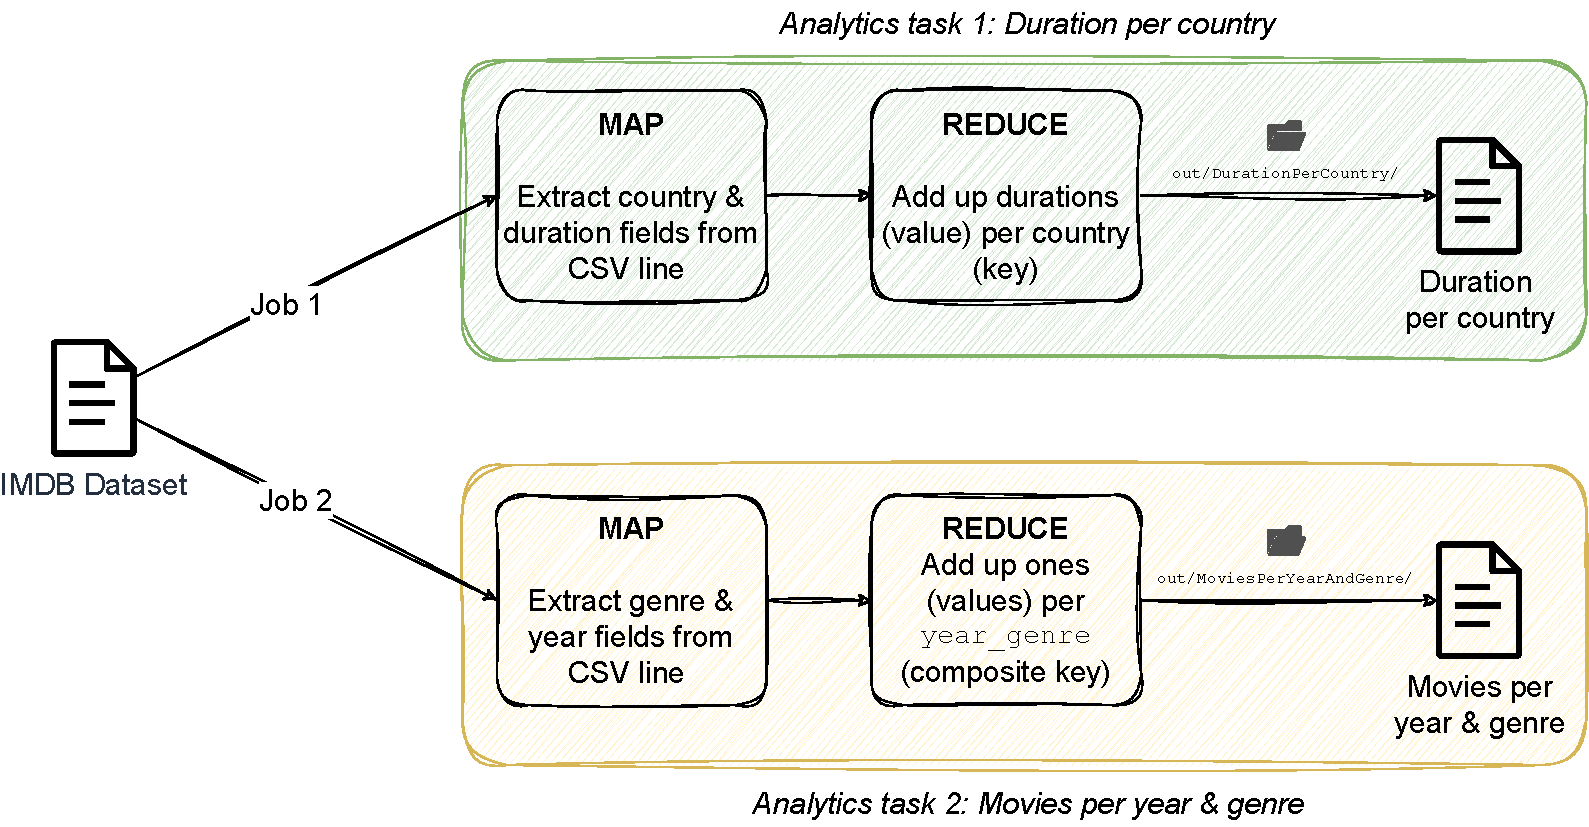
\includegraphics[width=0.8\linewidth]{figures/movieAnalytics}
  \caption{The MapReduce solution architecture for the movie analytics problem. Two separate jobs are executed to solve the two tasks, namely duration per country (green) and movies per year \& genre (yellow). The two tasks also create separate subdirectories for writing the results.}
  \label{img:movieAnalyticsSolutionDiagram}
\end{figure}

\paragraph{Task 1: Duration per country} One map-reduce cycle is enough to handle this task, as depicted in the top part of~\autoref{img:movieAnalyticsSolutionDiagram} in green color. The map function parses the CSV file line by line and extracts the useful fields from each line. In this case, the useful fields are the country (or countries) the movie was produced and the movie duration, i.e., the fourth and ninth fields in the input line respectively. We employ more complex logic to handle cases where there are multiple countries in a single movie. In particular, we parse again the field and tokenize it into the separate countries, producing a key-value pair for each country-duration pair within a movie. The reduce function is, then, trivial; it just adds up the durations (value) per country (key) and outputs the results. The interested reader can refer to the \texttt{CSVProcessor.java} (mapper), \texttt{AnayticsEngine.java} (reducer) and \texttt{MovieAnalyticsMaster.java} (driver) files for the source code implementation of our solution.

\paragraph{Task 2: Movies per year \& genre w.r.t. score constraint} The task is similar to the first one, with the only difference lying in the fields extracted from the input CSV line. In this case, we are interested about the year, the genre (or genres) and score fields, i.e., the third, fifth and seventh fields in the input CSV line. The map function produces key-value pairs in the form \texttt{(composite\_key, 1)}, where the composite key consists of the year and the genre of the respective movie concatenated by an underscore, e.g., \texttt{2024\_action}. We handle multiple genres per movie similarly with the multiple countries in task 1. We employ the same trivial reducer that adds up the values (ones) per (composite) key, as shown in the bottom part of~\autoref{img:movieAnalyticsSolutionDiagram} in yellow color.

\subsubsection{Evaluation} Our solution is tested using the provided IMDB dataset, namely \texttt{movies.csv}. We list the execution results in~\autoref{sec:data2}.

\section{Problem 3: DNA Sequence Patterns}
\label{sec:problem3}
The third problem focuses on mining unstructured data, namely DNA sequences, encoded in text format.


\subsection{Problem Statement}
A DNA sequence consists of four distinct symbols, namely A, G, C, and T. For instance, the following lines represent a part of the DNA sequence of the E. Coli bacterium~\footnote{\href{https://en.wikipedia.org/wiki/Pathogenic_Escherichia_coli}{https://en.wikipedia.org/wiki/Pathogenic\_Escherichia\_coli}}:

\begin{verbatim}
AGCTTTTCATTCTGACTGCAACGGGCAATATGTCTCTGTGTGGATTAAAAAAAGAGTGTCTGATAGCAGC
TTCTGAACTGGTTACCTGCCGTGAGTAAATTAAAATTTTATTGACTTAGGTCACTAAATACTTTAACCAA
TATAGGCATAGCGCACAGACAGATAAAAATTACAGAGTACACAACATCCATGAAACGCATTAGCACCACC
ATTACCACCACCATCACCATTACCACAGGTAACGGTGCGGGCTGACGCGTACAGGAAACACAGAAAAAAG
\end{verbatim}

Implement a \textbf{MapReduce} program that computes the frequency (i.e., number of occurrences) of all subsequences of lengths 2, 3, and 4 that are present in the input DNA sequence. Note that the processing of each line should be independent of all other lines. Use the file \texttt{ecoli.txt} to test your solution.

\subsection{Proposed approach}
\subsubsection{Setting}
Our implementation is run and tested in a Linux environment with 12 cores, using the Java programming language.
We have used the Java Development Kit (JDK) version 11.0.11.
The source code is developed in IntelliJ IDEA Community Edition 2021.1.1 and managed using Maven as the build tool.

The project’s dependencies, including Hadoop libraries, are defined in the \texttt{pom.xml} file located in the root of
the repository.
The project is compiled and executed directly from IntelliJ IDEA.
To run the project, open the \texttt{DNASequenceAnalyticsMaster} class in IntelliJ IDEA, and execute the main method.
You will need to specify the following command-line arguments:

\begin{itemize}
  \item \texttt{<input\_path>} specifies the directory containing the input text files, located at \texttt{map-reduce/ \\ dnaSequencePatterns/input}.
  \item \texttt{<output\_path>} specifies the directory where the MapReduce output will be written, which will be created in the \texttt{out} folder.
\end{itemize}

IntelliJ IDEA will handle the compilation and execution automatically when the main method is run. Make sure to configure the input and output paths as required for your specific run. Note that the command-line arguments must follow the specified order and format. If any of the arguments are missing or invalid, the program will terminate with an appropriate error message.

\subsubsection{Implementation} \autoref{algo:subsequences} summarizes the most substantial part of our implementation, namely the logic that is implemented inside the mappers of our solution. At every execution of the map function, a DNA sequence line is given as input to the mapper. The latter is responsible for populating all possible subsequences of length 2, 3 and 4. We employ a sliding window that is nested inside a for-loop defining the subsequence length. The source code implementation of~\autoref{algo:subsequences} can be found in the \texttt{DNASequenceProcessor.java} file.

\begin{algorithm}[!tb]
  \caption{Populating DNA subsequences}
  \label{algo:subsequences}
  \begin{algorithmic}[1]
    \LComment{Input: a DNA sequence $line$ (variable line)}
    \For{$length \in \{2, 3, 4\}$}
    \State Create a sliding window $window$ of length $length$.
    \State Place left end of $window$ at the start of $line$.
    \While{right end of $window$ has not exceeded $line$}
    \State $subsequence \gets$ contents of $window$
    \State Yield $(subsequence, 1)$ key-value pair.
    \State Slide window to the right by $1$.
    \EndWhile
    \EndFor
  \end{algorithmic}
\end{algorithm}

\subsubsection{Evaluation} Our solution is tested using the provided DNA sequence, namely \texttt{ecoli.txt}. We list the execution results in~\autoref{sec:data3}.

\section{Problem 4: Probabilistic graph}
\label{sec:problem4}
We discuss here the fourth problem of the assignment.
The main target of the assignment is to get acquainted with performing various MapReduce phases on a pipeline frame.

\subsection{Problem Statement}
We are given an input file in text format where each line contains a connection between two vertices of a network and a
probability value.
For each edge \( e \), there is a probability value \( p(e) \) which indicates the probability that the two vertices are
connected by the edge.
Obviously, the values of \( p(e) \) range between 0 and 1.
The values in each line are separated by a space.
Consider the network shown in the previous figure.
The edge connecting vertices 4 and 5 has a probability of
0.8, the edge connecting vertices 2 and 3 has a probability of 0.2, etc.

\begin{figure}[h]
  \centering
  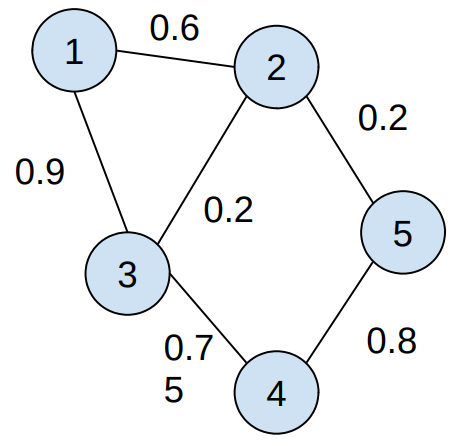
\includegraphics[width=0.25\linewidth]{figures/graph}
\end{figure}

The file corresponding to this graph would be:

\[
  1 \ 2 \ 0.6, \\
  1 \ 3 \ 0.9, \\
  2 \ 3 \ 0.2, \\
  3 \ 4 \ 0.75, \\
  2 \ 5 \ 0.2, \\
  4 \ 5 \ 0.8,
\]

The edges are generally stored in random order in the file, so we cannot assume they have a specific arrangement.

The following tasks are requested:

\begin{enumerate}
  \item Write a Java program that computes the average degree for all the vertices.
  \item The average degree is defined as the sum of the probabilities of the edges that fall on a vertex.
  \item For example, in the previous diagram, the average degree of vertex 3 is \( 0.9 + 0.2 + 0.75 = 1.85 \).
  \item Before performing this calculation, you should ignore all edges with a probability less than a threshold \( T \)
        , which should be passed as a parameter to the main function.
  \item Modify the code from task 1 so that, at the end, only the vertices with an average degree greater than the
        average of the degrees of all the vertices are displayed in the output.

\end{enumerate}

\subsection{Proposed approach}
\subsubsection{Setting}
Our implementation is run and tested in a Linux environment with 12 cores, using the Java programming language.
We have used the Java Development Kit (JDK) version 11.0.11.
The source code is developed in IntelliJ IDEA Community Edition 2021.1.1 and managed using Maven as the build tool.

The project’s dependencies, including Hadoop libraries, are defined in the \texttt{pom.xml} file located in the root of
the repository.
The project is compiled and executed directly from IntelliJ IDEA.

To run the project, open the \texttt{GraphMaster} class in IntelliJ IDEA, and execute the main method.
You will need to specify the following command-line arguments:

\begin{itemize}
  \item \texttt{<input\_path>} specifies the directory containing the input text files, located at
        \texttt{map-reduce/ probabilisticGraph /input}.
  \item \texttt{<output\_path>} specifies the directory where the MapReduce output will be written, which will be
        created in the \texttt{out} folder.
  \item \texttt{<T>} is the minimum edge-degree threshold for vertices to be included in the results.
\end{itemize}

IntelliJ IDEA will handle the compilation and execution automatically when the main method is run.
Make sure to configure the input and output paths as required for your specific run.

Note that the command-line arguments must follow the specified order and format.
If any of the arguments are missing or invalid, the program will terminate with an appropriate error message.

\subsubsection{Implementation}
The problem at hand involves processing a probabilistic graph, where each edge connects two vertices with a probability
value.
The task is to compute the average degree for each vertex, considering only edges whose probability exceeds a given
threshold \( T \).
The methodology proposed here utilizes a distributed MapReduce framework, implemented using Hadoop, to efficiently
process and analyze large-scale graph data.
The approach is divided into three main phases, each handled by separate MapReduce jobs, with intermediate results
passed between the phases.

The \texttt{GraphMaster} class serves as the orchestrator of the entire MapReduce process.
It manages the execution of the three phases, invoking the appropriate MapReduce jobs in sequence.
The main steps executed by \texttt{GraphMaster} are:

\begin{enumerate}
  \item It retrieves the command-line arguments, including the input and output directories as well as the threshold
        value \( T \), which determines which edges to consider in the graph.
  \item It initiates the first MapReduce job to compute the degree of each vertex in the graph.
        The input consists of edge data, and the output is a summation of edge probabilities for each vertex.
  \item After the first job completes, the \texttt{GraphMaster} starts the second MapReduce job to calculate the mean
        degree of the graph, using the results from the first job.
  \item Once the mean degree is computed, \texttt{GraphMaster} starts the third MapReduce job, which filters out the
        vertices with degrees lower than the mean degree.
  \item It cleans up intermediate directories after each phase and moves the final output to the desired location.
\end{enumerate}

\texttt{GraphMaster} coordinates these steps by configuring and executing the MapReduce jobs, ensuring that each phase
depends on the results of the previous one. \\

The entire process consists of three MapReduce jobs, executed sequentially:

\begin{enumerate}
  \item \textbf{Phase 1:} The first job computes the degree of each vertex by summing the probabilities of the edges
        connected to it.
        It produces intermediate results for each vertex.
  \item \textbf{Phase 2:} The second job calculates the mean degree by summing the degrees from the first phase and
        dividing by the total number of vertices.
  \item \textbf{Phase 3:} The third job filters out the vertices with a degree lower than the mean degree and produces
        the final filtered result.
\end{enumerate}

After each job completes, intermediate data is written to disk and passed as input to the subsequent job.
The final output consists of the vertices whose degree exceeds or equals the mean degree. \\

\textbf{Phase 1: Calculating Vertex Degree}
The first MapReduce job is responsible for calculating the degree of each vertex in the graph, where the degree is
defined as the sum of the probabilities of the edges connected to that vertex.
The degree of each vertex is computed by the \texttt{GraphMapper} and \texttt{GraphReducer} classes.

The \texttt{GraphMapper} class reads each edge from the input data, which consists of lines containing two vertices
and the associated probability value.
It splits each line into two components (the two vertices), and for each vertex, it emits the corresponding probability
value as the output.
The mapper also checks if the probability value exceeds the threshold \( T \), which is provided as a configuration
parameter.
If the probability is greater than or equal to \( T \), it emits the vertex along with the corresponding probability.

The \texttt{GraphReducer} class receives the vertex and associated probability values emitted by the mapper.
For each vertex, it sums up all the probabilities of the edges connected to that vertex, and emits the pair as output.

\textbf{Phase 2: Calculating the Mean Degree}
The second phase of the approach calculates the mean degree of all vertices.
This is done by summing the degree values from the previous phase and dividing by the total number of vertices.

The \texttt{MeanMapper} class receives the degree values from the output of the first MapReduce job.
It emits two key-value pairs for each input line: a count of the number of vertices and the sum of the degree values.
These are emitted with fixed keys (\texttt{"count"} and \texttt{"sum"}) so that they can be aggregated in the reducer.

The \texttt{MeanReducer} class processes the count and sum values emitted by the mapper.
It calculates the total sum and count of vertices and then writes these values as output.
The mean degree is calculated by dividing the sum by the count, and the result is stored for use in the next phase.

\textbf{Phase 3: Filtering Vertices by Mean Degree}
In the third phase, the vertices whose degree is greater than or equal to the mean degree calculated in Phase 2 are
selected.
This phase uses the results from Phase 1 and Phase 2, applying the filtering criteria to retain only those vertices with
a degree greater than or equal to the mean.

The \texttt{FilterMapper} class takes the degree values emitted by the first reducer and writes them as key-value pairs.
Each key is a vertex, and the value is the degree of that vertex.
The mapper does not perform any filtering; instead, it simply passes the values along to the reducer.

The \texttt{FilterReducer} class filters out the vertices whose degree is less than the mean degree.
It retrieves the mean degree from the configuration, and for each vertex, it compares the degree value to the mean.
If the degree is greater than or equal to the mean, it emits the vertex along with its degree.
This final output contains only the vertices that satisfy the filtering criteria.

\subsubsection{Evaluation}
The experiments were executed using the dataset `collins.txt` with a parameter setting of \( T = 0.8 \).

To provide a comprehensive overview, the results of the experiment, including the detailed values derived from the
dataset, are presented in~\autoref{sec:data4} in a 2-column format.



\section{Conclusion}
\label{sec:conclusion}
TODO: In this document we have presented our solutions and rational for solving the first assignment of the M.Sc.
course
on \emph{Technologies for Big Data Analysis}, offered by the \emph{DWS M.Sc. Program}.

\appendix
\section{Problem 1}
\label{sec:data1}
In the following 8-columned pages, the experimental results of section's  \ref{sec:problem1} problem are presented,
as the raw output of the MapReduce execution.

\begin{multicols}{8}
  \noindent
  a10c: 34
  \\ a10d: 486
  \\ a10e: 386
  \\ a10g: 175
  \\ a10h: 58
  \\ a10l: 131
  \\ a10m: 15
  \\ a10n: 260
  \\ a10p: 48
  \\ a10r: 68
  \\ a10s: 429
  \\ a10t: 72
  \\ a10y: 190
  \\ a10z: 50
  \\ a11a: 36
  \\ a11c: 36
  \\ a11d: 165
  \\ a11e: 136
  \\ a11g: 101
  \\ a11n: 202
  \\ a11p: 16
  \\ a11r: 13
  \\ a11s: 266
  \\ a11t: 115
  \\ a11y: 119
  \\ a12c: 18
  \\ a12d: 94
  \\ a12e: 95
  \\ a12g: 47
  \\ a12l: 20
  \\ a12n: 65
  \\ a12s: 139
  \\ a12t: 59
  \\ a12y: 36
  \\ a13e: 10
  \\ a13g: 19
  \\ a13n: 22
  \\ a13s: 112
  \\ a13t: 36
  \\ a13y: 36
  \\ a14c: 12
  \\ a14e: 16
  \\ a14n: 114
  \\ a14s: 16
  \\ a14t: 17
  \\ a14y: 38
  \\ a15s: 33
  \\ a16s: 18
  \\ a3d: 38224
  \\ a3e: 3767
  \\ a3k: 248
  \\ a3l: 4077
  \\ a3m: 353
  \\ a3o: 106
  \\ a3r: 198
  \\ a3t: 428
  \\ a3y: 1193
  \\ a4a: 458
  \\ a4d: 166
  \\ a4e: 249
  \\ a4h: 13
  \\ a4n: 15
  \\ a4o: 773
  \\ a4s: 483
  \\ a4t: 47
  \\ a4y: 1588
  \\ a5a: 41
  \\ a5d: 1360
  \\ a5e: 1377
  \\ a5g: 841
  \\ a5i: 11
  \\ a5l: 112
  \\ a5m: 56
  \\ a5n: 916
  \\ a5r: 1604
  \\ a5s: 213
  \\ a5t: 1767
  \\ a5w: 94
  \\ a5y: 201
  \\ a6a: 112
  \\ a6d: 785
  \\ a6e: 615
  \\ a6g: 214
  \\ a6h: 21
  \\ a6k: 151
  \\ a6l: 192
  \\ a6m: 20
  \\ a6n: 456
  \\ a6p: 84
  \\ a6r: 523
  \\ a6s: 1197
  \\ a6t: 811
  \\ a6w: 1078
  \\ a6y: 204
  \\ a7a: 431
  \\ a7c: 52
  \\ a7d: 1076
  \\ a7e: 685
  \\ a7g: 71
  \\ a7h: 12
  \\ a7l: 116
  \\ a7n: 83
  \\ a7r: 843
  \\ a7s: 1203
  \\ a7t: 1011
  \\ a7x: 17
  \\ a7y: 756
  \\ a8a: 28
  \\ a8c: 37
  \\ a8d: 1790
  \\ a8e: 386
  \\ a8g: 625
  \\ a8h: 328
  \\ a8l: 125
  \\ a8m: 239
  \\ a8n: 982
  \\ a8r: 98
  \\ a8s: 469
  \\ a8t: 440
  \\ a8x: 10
  \\ a8y: 328
  \\ a9a: 27
  \\ a9c: 23
  \\ a9d: 531
  \\ a9e: 369
  \\ a9g: 548
  \\ a9l: 62
  \\ a9n: 555
  \\ a9r: 235
  \\ a9s: 622
  \\ a9t: 287
  \\ a9v: 38
  \\ a9y: 286
  \\ b10a: 17
  \\ b10d: 86
  \\ b10e: 58
  \\ b10g: 28
  \\ b10l: 20
  \\ b10m: 12
  \\ b10n: 13
  \\ b10r: 33
  \\ b10s: 227
  \\ b10t: 43
  \\ b10y: 10
  \\ b11a: 10
  \\ b11d: 79
  \\ b11g: 15
  \\ b11m: 34
  \\ b11n: 21
  \\ b11o: 48
  \\ b11s: 75
  \\ b11t: 13
  \\ b11y: 19
  \\ b12d: 36
  \\ b12e: 20
  \\ b12g: 10
  \\ b12l: 18
  \\ b12s: 25
  \\ b12t: 10
  \\ b12w: 10
  \\ b12y: 21
  \\ b13e: 10
  \\ b13v: 13
  \\ b3d: 352
  \\ b3e: 11
  \\ b3g: 145
  \\ b3r: 22
  \\ b3t: 5674
  \\ b3w: 35
  \\ b3x: 66
  \\ b3y: 223
  \\ b4d: 268
  \\ b4e: 883
  \\ b4f: 10
  \\ b4g: 96
  \\ b4h: 538
  \\ b4k: 969
  \\ b4l: 288
  \\ b4m: 16
  \\ b4n: 2688
  \\ b4r: 102
  \\ b4s: 119
  \\ b4t: 458
  \\ b4w: 98
  \\ b4y: 459
  \\ b5a: 77
  \\ b5d: 934
  \\ b5e: 330
  \\ b5f: 29
  \\ b5g: 1080
  \\ b5h: 103
  \\ b5k: 342
  \\ b5l: 11
  \\ b5m: 29
  \\ b5n: 1190
  \\ b5r: 60
  \\ b5s: 1288
  \\ b5t: 212
  \\ b5w: 111
  \\ b5y: 101
  \\ b6a: 42
  \\ b6d: 865
  \\ b6e: 3041
  \\ b6f: 52
  \\ b6g: 84
  \\ b6h: 123
  \\ b6i: 20
  \\ b6l: 39
  \\ b6m: 41
  \\ b6n: 329
  \\ b6r: 436
  \\ b6s: 390
  \\ b6t: 347
  \\ b6u: 17
  \\ b6w: 15
  \\ b6y: 181
  \\ b7a: 31
  \\ b7c: 25
  \\ b7d: 248
  \\ b7e: 1005
  \\ b7g: 339
  \\ b7h: 371
  \\ b7i: 31
  \\ b7k: 28
  \\ b7l: 16
  \\ b7m: 61
  \\ b7n: 861
  \\ b7o: 15
  \\ b7r: 238
  \\ b7s: 741
  \\ b7t: 494
  \\ b7u: 16
  \\ b7y: 196
  \\ b8a: 121
  \\ b8d: 308
  \\ b8e: 83
  \\ b8g: 451
  \\ b8h: 15
  \\ b8l: 55
  \\ b8m: 41
  \\ b8n: 53
  \\ b8o: 105
  \\ b8r: 55
  \\ b8s: 795
  \\ b8t: 62
  \\ b8v: 148
  \\ b8y: 78
  \\ b9a: 26
  \\ b9d: 95
  \\ b9e: 232
  \\ b9g: 271
  \\ b9h: 18
  \\ b9i: 161
  \\ b9l: 175
  \\ b9n: 274
  \\ b9r: 19
  \\ b9s: 163
  \\ b9t: 150
  \\ b9y: 19
  \\ c10a: 49
  \\ c10d: 460
  \\ c10e: 395
  \\ c10g: 362
  \\ c10l: 129
  \\ c10n: 689
  \\ c10r: 18
  \\ c10s: 818
  \\ c10t: 97
  \\ c10y: 256
  \\ c11a: 21
  \\ c11d: 116
  \\ c11e: 272
  \\ c11g: 141
  \\ c11l: 92
  \\ c11n: 403
  \\ c11p: 12
  \\ c11r: 16
  \\ c11s: 341
  \\ c11t: 74
  \\ c11y: 181
  \\ c12d: 107
  \\ c12e: 284
  \\ c12g: 46
  \\ c12h: 11
  \\ c12l: 15
  \\ c12n: 673
  \\ c12r: 10
  \\ c12s: 173
  \\ c12t: 45
  \\ c12y: 124
  \\ c13d: 80
  \\ c13e: 35
  \\ c13g: 61
  \\ c13l: 29
  \\ c13n: 220
  \\ c13s: 379
  \\ c13y: 83
  \\ c14a: 14
  \\ c14c: 94
  \\ c14e: 47
  \\ c14l: 93
  \\ c14n: 20
  \\ c14s: 84
  \\ c14y: 29
  \\ c15d: 11
  \\ c15e: 12
  \\ c15s: 24
  \\ c15y: 18
  \\ c16e: 39
  \\ c16f: 10
  \\ c3b: 34
  \\ c3n: 872
  \\ c3p: 117
  \\ c3t: 210
  \\ c3y: 140
  \\ c4a: 35
  \\ c4b: 72
  \\ c4d: 333
  \\ c4e: 2548
  \\ c4f: 18
  \\ c4k: 36
  \\ c4l: 246
  \\ c4m: 88
  \\ c4n: 92
  \\ c4p: 105
  \\ c4r: 31
  \\ c4s: 42
  \\ c4t: 739
  \\ c4w: 12
  \\ c4y: 285
  \\ c5a: 45
  \\ c5c: 10
  \\ c5d: 2428
  \\ c5e: 804
  \\ c5f: 320
  \\ c5g: 24
  \\ c5h: 168
  \\ c5i: 18
  \\ c5k: 237
  \\ c5l: 318
  \\ c5m: 77
  \\ c5n: 161
  \\ c5p: 33
  \\ c5r: 479
  \\ c5s: 1360
  \\ c5t: 1031
  \\ c5y: 130
  \\ c6a: 44
  \\ c6c: 40
  \\ c6d: 871
  \\ c6e: 1144
  \\ c6g: 247
  \\ c6h: 125
  \\ c6l: 61
  \\ c6m: 30
  \\ c6n: 676
  \\ c6r: 706
  \\ c6s: 929
  \\ c6t: 568
  \\ c6x: 23
  \\ c6y: 363
  \\ c7a: 23
  \\ c7c: 148
  \\ c7d: 1329
  \\ c7e: 561
  \\ c7g: 328
  \\ c7h: 15
  \\ c7k: 80
  \\ c7l: 690
  \\ c7m: 35
  \\ c7n: 703
  \\ c7o: 27
  \\ c7r: 658
  \\ c7s: 834
  \\ c7t: 612
  \\ c7x: 23
  \\ c7y: 1192
  \\ c8a: 125
  \\ c8c: 46
  \\ c8d: 582
  \\ c8e: 638
  \\ c8g: 570
  \\ c8h: 26
  \\ c8l: 573
  \\ c8n: 523
  \\ c8o: 18
  \\ c8r: 285
  \\ c8s: 2081
  \\ c8t: 341
  \\ c8x: 16
  \\ c8y: 394
  \\ c9a: 39
  \\ c9d: 1289
  \\ c9e: 440
  \\ c9g: 137
  \\ c9l: 41
  \\ c9m: 42
  \\ c9n: 616
  \\ c9r: 485
  \\ c9s: 836
  \\ c9t: 198
  \\ c9v: 10
  \\ c9y: 381
  \\ d10a: 113
  \\ d10c: 142
  \\ d10d: 345
  \\ d10e: 169
  \\ d10g: 194
  \\ d10l: 29
  \\ d10n: 175
  \\ d10r: 15
  \\ d10s: 211
  \\ d10t: 120
  \\ d10v: 44
  \\ d10y: 259
  \\ d11a: 13
  \\ d11d: 205
  \\ d11e: 106
  \\ d11g: 78
  \\ d11h: 32
  \\ d11l: 23
  \\ d11m: 17
  \\ d11n: 352
  \\ d11s: 176
  \\ d11t: 121
  \\ d11y: 63
  \\ d12d: 112
  \\ d12e: 70
  \\ d12g: 44
  \\ d12l: 21
  \\ d12n: 162
  \\ d12s: 168
  \\ d12t: 32
  \\ d12y: 37
  \\ d13d: 84
  \\ d13e: 52
  \\ d13g: 13
  \\ d13n: 63
  \\ d13s: 29
  \\ d13t: 13
  \\ d14d: 17
  \\ d14g: 16
  \\ d14n: 27
  \\ d14s: 10
  \\ d14t: 11
  \\ d14y: 13
  \\ d15n: 31
  \\ d15s: 19
  \\ d3c: 10
  \\ d3d: 1874
  \\ d3e: 335
  \\ d3g: 71
  \\ d3m: 55
  \\ d3n: 29
  \\ d3s: 11
  \\ d3y: 882
  \\ d4a: 19
  \\ d4d: 284
  \\ d4e: 602
  \\ d4g: 27
  \\ d4h: 19
  \\ d4k: 187
  \\ d4l: 170
  \\ d4m: 29
  \\ d4n: 1183
  \\ d4p: 258
  \\ d4r: 935
  \\ d4s: 900
  \\ d4t: 713
  \\ d4u: 19
  \\ d4w: 203
  \\ d4y: 161
  \\ d5a: 11
  \\ d5d: 114
  \\ d5e: 296
  \\ d5g: 250
  \\ d5h: 374
  \\ d5k: 109
  \\ d5l: 77
  \\ d5m: 43
  \\ d5n: 209
  \\ d5s: 415
  \\ d5t: 305
  \\ d5y: 245
  \\ d6a: 39
  \\ d6d: 313
  \\ d6e: 549
  \\ d6g: 566
  \\ d6h: 10
  \\ d6i: 14
  \\ d6l: 146
  \\ d6m: 27
  \\ d6n: 177
  \\ d6r: 617
  \\ d6s: 281
  \\ d6t: 341
  \\ d6y: 154
  \\ d7b: 13
  \\ d7c: 21
  \\ d7d: 989
  \\ d7e: 1011
  \\ d7g: 439
  \\ d7l: 18
  \\ d7n: 43
  \\ d7o: 10
  \\ d7p: 56
  \\ d7r: 107
  \\ d7s: 665
  \\ d7t: 220
  \\ d7v: 366
  \\ d7y: 183
  \\ d8a: 46
  \\ d8c: 93
  \\ d8d: 903
  \\ d8e: 536
  \\ d8g: 305
  \\ d8h: 52
  \\ d8k: 15
  \\ d8l: 119
  \\ d8m: 37
  \\ d8n: 272
  \\ d8r: 296
  \\ d8s: 475
  \\ d8t: 183
  \\ d8v: 284
  \\ d8y: 138
  \\ d9a: 31
  \\ d9d: 793
  \\ d9e: 326
  \\ d9g: 169
  \\ d9m: 14
  \\ d9n: 202
  \\ d9r: 48
  \\ d9s: 855
  \\ d9t: 470
  \\ d9v: 26
  \\ d9y: 257
  \\ e10c: 57
  \\ e10d: 104
  \\ e10e: 256
  \\ e10g: 553
  \\ e10h: 23
  \\ e10l: 67
  \\ e10m: 91
  \\ e10n: 431
  \\ e10s: 136
  \\ e10t: 195
  \\ e10y: 610
  \\ e11a: 49
  \\ e11d: 331
  \\ e11e: 20
  \\ e11g: 29
  \\ e11l: 62
  \\ e11m: 20
  \\ e11n: 195
  \\ e11s: 134
  \\ e11t: 95
  \\ e11y: 115
  \\ e12a: 11
  \\ e12c: 16
  \\ e12d: 49
  \\ e12g: 79
  \\ e12l: 13
  \\ e12n: 38
  \\ e12s: 88
  \\ e12t: 23
  \\ e12y: 20
  \\ e13n: 15
  \\ e13s: 59
  \\ e13t: 75
  \\ e13y: 91
  \\ e14g: 10
  \\ e14s: 24
  \\ e14y: 14
  \\ e3a: 11
  \\ e3c: 18
  \\ e3d: 456
  \\ e3e: 137
  \\ e3r: 45
  \\ e3t: 67
  \\ e4a: 12
  \\ e4e: 304
  \\ e4h: 409
  \\ e4l: 53
  \\ e4n: 941
  \\ e4r: 253
  \\ e4s: 1113
  \\ e4t: 149
  \\ e4y: 129
  \\ e5a: 13
  \\ e5d: 43
  \\ e5e: 56
  \\ e5h: 117
  \\ e5k: 85
  \\ e5l: 164
  \\ e5n: 46
  \\ e5r: 210
  \\ e5s: 98
  \\ e5t: 327
  \\ e5w: 87
  \\ e5y: 1240
  \\ e6a: 13
  \\ e6d: 174
  \\ e6e: 651
  \\ e6g: 39
  \\ e6h: 189
  \\ e6i: 12
  \\ e6m: 10
  \\ e6n: 28
  \\ e6r: 335
  \\ e6s: 496
  \\ e6t: 710
  \\ e6y: 213
  \\ e7a: 18
  \\ e7c: 69
  \\ e7d: 1198
  \\ e7e: 588
  \\ e7g: 279
  \\ e7h: 213
  \\ e7l: 29
  \\ e7m: 11
  \\ e7n: 255
  \\ e7o: 10
  \\ e7r: 569
  \\ e7s: 575
  \\ e7t: 209
  \\ e7v: 28
  \\ e7y: 234
  \\ e8a: 11
  \\ e8c: 152
  \\ e8d: 864
  \\ e8e: 572
  \\ e8g: 232
  \\ e8l: 107
  \\ e8m: 19
  \\ e8n: 348
  \\ e8r: 62
  \\ e8s: 531
  \\ e8t: 40
  \\ e8y: 174
  \\ e9c: 42
  \\ e9d: 544
  \\ e9e: 386
  \\ e9g: 244
  \\ e9h: 75
  \\ e9l: 122
  \\ e9n: 283
  \\ e9r: 31
  \\ e9s: 330
  \\ e9t: 153
  \\ e9y: 634
  \\ f10d: 228
  \\ f10e: 83
  \\ f10g: 95
  \\ f10h: 29
  \\ f10n: 128
  \\ f10p: 42
  \\ f10r: 20
  \\ f10s: 124
  \\ f10t: 63
  \\ f10v: 12
  \\ f10y: 242
  \\ f11d: 19
  \\ f11e: 46
  \\ f11g: 73
  \\ f11l: 21
  \\ f11n: 42
  \\ f11s: 142
  \\ f11t: 15
  \\ f11y: 59
  \\ f12g: 14
  \\ f12n: 11
  \\ f12s: 33
  \\ f13s: 10
  \\ f3d: 18
  \\ f3e: 47
  \\ f3g: 340
  \\ f3n: 26
  \\ f3o: 17
  \\ f3r: 7246
  \\ f3t: 128
  \\ f3w: 453
  \\ f3x: 44
  \\ f3y: 33
  \\ f4d: 493
  \\ f4e: 2351
  \\ f4g: 31
  \\ f4h: 16
  \\ f4i: 27
  \\ f4k: 35
  \\ f4l: 859
  \\ f4m: 6376
  \\ f4p: 28
  \\ f4r: 444
  \\ f4s: 73
  \\ f4t: 1443
  \\ f4w: 96
  \\ f4x: 11
  \\ f4y: 21
  \\ f5a: 22
  \\ f5d: 1113
  \\ f5e: 402
  \\ f5g: 32
  \\ f5h: 404
  \\ f5k: 140
  \\ f5l: 132
  \\ f5n: 23
  \\ f5r: 353
  \\ f5s: 867
  \\ f5t: 1749
  \\ f5y: 346
  \\ f6a: 61
  \\ f6d: 958
  \\ f6e: 500
  \\ f6g: 183
  \\ f6h: 1159
  \\ f6l: 60
  \\ f6n: 122
  \\ f6o: 13
  \\ f6r: 892
  \\ f6s: 520
  \\ f6t: 319
  \\ f6w: 344
  \\ f6y: 435
  \\ f7a: 76
  \\ f7d: 590
  \\ f7e: 324
  \\ f7g: 756
  \\ f7h: 48
  \\ f7l: 282
  \\ f7m: 220
  \\ f7n: 410
  \\ f7r: 333
  \\ f7s: 1066
  \\ f7t: 43
  \\ f7y: 265
  \\ f8d: 604
  \\ f8e: 190
  \\ f8g: 218
  \\ f8h: 39
  \\ f8k: 11
  \\ f8l: 56
  \\ f8m: 21
  \\ f8n: 226
  \\ f8r: 152
  \\ f8s: 473
  \\ f8t: 118
  \\ f8y: 223
  \\ f9a: 17
  \\ f9c: 12
  \\ f9d: 147
  \\ f9e: 131
  \\ f9g: 266
  \\ f9h: 26
  \\ f9k: 31
  \\ f9l: 51
  \\ f9n: 454
  \\ f9o: 16
  \\ f9r: 24
  \\ f9s: 309
  \\ f9t: 53
  \\ f9y: 59
  \\ g10a: 20
  \\ g10d: 16
  \\ g10g: 52
  \\ g10n: 37
  \\ g10r: 12
  \\ g10s: 120
  \\ g10t: 643
  \\ g10y: 40
  \\ g11d: 60
  \\ g11g: 22
  \\ g11l: 21
  \\ g11m: 126
  \\ g11n: 89
  \\ g11r: 20
  \\ g11s: 71
  \\ g12d: 10
  \\ g12l: 16
  \\ g12s: 74
  \\ g13y: 10
  \\ g14g: 10
  \\ g18g: 13
  \\ g3d: 305
  \\ g3m: 13
  \\ g3n: 54
  \\ g3p: 44
  \\ g3s: 11
  \\ g3t: 752
  \\ g3y: 33
  \\ g4d: 855
  \\ g4e: 1349
  \\ g4f: 13
  \\ g4l: 185
  \\ g4m: 20
  \\ g4n: 91
  \\ g4p: 14
  \\ g4s: 269
  \\ g4t: 44
  \\ g4w: 255
  \\ g4y: 110
  \\ g5a: 40
  \\ g5d: 278
  \\ g5e: 276
  \\ g5f: 47
  \\ g5g: 369
  \\ g5h: 15
  \\ g5i: 10
  \\ g5m: 59
  \\ g5n: 594
  \\ g5p: 168
  \\ g5s: 549
  \\ g5t: 935
  \\ g5y: 136
  \\ g6a: 13
  \\ g6d: 281
  \\ g6e: 336
  \\ g6g: 256
  \\ g6h: 223
  \\ g6l: 22
  \\ g6n: 305
  \\ g6p: 63
  \\ g6r: 47
  \\ g6s: 717
  \\ g6t: 10
  \\ g6y: 229
  \\ g7a: 83
  \\ g7d: 366
  \\ g7e: 126
  \\ g7g: 314
  \\ g7h: 19
  \\ g7l: 848
  \\ g7m: 25
  \\ g7n: 29
  \\ g7p: 15
  \\ g7r: 167
  \\ g7s: 328
  \\ g7t: 31
  \\ g7y: 216
  \\ g8c: 29
  \\ g8d: 221
  \\ g8e: 185
  \\ g8g: 232
  \\ g8l: 37
  \\ g8n: 73
  \\ g8r: 139
  \\ g8s: 306
  \\ g8t: 83
  \\ g8y: 37
  \\ g9a: 19
  \\ g9d: 33
  \\ g9e: 65
  \\ g9g: 188
  \\ g9n: 179
  \\ g9r: 45
  \\ g9s: 160
  \\ g9t: 37
  \\ g9y: 190
  \\ h10a: 55
  \\ h10c: 17
  \\ h10d: 35
  \\ h10e: 22
  \\ h10g: 26
  \\ h10h: 21
  \\ h10l: 76
  \\ h10n: 44
  \\ h10s: 207
  \\ h10y: 38
  \\ h11a: 19
  \\ h11c: 13
  \\ h11d: 17
  \\ h11e: 143
  \\ h11g: 21
  \\ h11n: 16
  \\ h11s: 32
  \\ h11y: 13
  \\ h12a: 17
  \\ h12c: 12
  \\ h12f: 55
  \\ h12g: 12
  \\ h12s: 90
  \\ h13d: 13
  \\ h13s: 20
  \\ h3d: 7393
  \\ h3e: 11
  \\ h3m: 5193
  \\ h3p: 37
  \\ h3r: 5252
  \\ h3s: 11727
  \\ h3t: 268
  \\ h3w: 1296
  \\ h3y: 47
  \\ h4d: 2139
  \\ h4e: 4797
  \\ h4f: 251
  \\ h4g: 59
  \\ h4h: 286
  \\ h4k: 11
  \\ h4l: 277
  \\ h4m: 38
  \\ h4n: 22
  \\ h4o: 53
  \\ h4p: 259
  \\ h4r: 557
  \\ h4s: 66
  \\ h4t: 229
  \\ h4y: 50
  \\ h5d: 709
  \\ h5e: 1028
  \\ h5h: 23
  \\ h5i: 10
  \\ h5l: 22
  \\ h5n: 184
  \\ h5o: 10
  \\ h5r: 193
  \\ h5s: 1072
  \\ h5t: 311
  \\ h5y: 509
  \\ h6a: 30
  \\ h6c: 33
  \\ h6d: 321
  \\ h6e: 212
  \\ h6g: 718
  \\ h6h: 170
  \\ h6i: 14
  \\ h6n: 214
  \\ h6r: 443
  \\ h6s: 1051
  \\ h6t: 96
  \\ h6w: 55
  \\ h6y: 274
  \\ h7a: 16
  \\ h7d: 544
  \\ h7e: 44
  \\ h7f: 1487
  \\ h7g: 535
  \\ h7h: 13
  \\ h7l: 48
  \\ h7m: 25
  \\ h7n: 48
  \\ h7r: 466
  \\ h7s: 490
  \\ h7t: 118
  \\ h7y: 683
  \\ h8c: 47
  \\ h8d: 313
  \\ h8e: 182
  \\ h8g: 47
  \\ h8h: 10
  \\ h8l: 66
  \\ h8n: 150
  \\ h8o: 22
  \\ h8s: 254
  \\ h8t: 33
  \\ h8y: 89
  \\ h9a: 19
  \\ h9c: 10
  \\ h9d: 139
  \\ h9e: 136
  \\ h9g: 70
  \\ h9k: 10
  \\ h9n: 61
  \\ h9s: 256
  \\ h9t: 18
  \\ h9y: 121
  \\ i10d: 309
  \\ i10e: 645
  \\ i10g: 134
  \\ i10l: 234
  \\ i10n: 306
  \\ i10s: 253
  \\ i10t: 99
  \\ i10y: 163
  \\ i11d: 212
  \\ i11e: 172
  \\ i11g: 127
  \\ i11l: 15
  \\ i11m: 10
  \\ i11n: 300
  \\ i11r: 23
  \\ i11s: 229
  \\ i11t: 191
  \\ i11y: 354
  \\ i12d: 19
  \\ i12e: 359
  \\ i12g: 33
  \\ i12l: 55
  \\ i12n: 505
  \\ i12s: 141
  \\ i12t: 52
  \\ i12y: 145
  \\ i13e: 100
  \\ i13l: 51
  \\ i13n: 35
  \\ i13r: 20
  \\ i13s: 32
  \\ i13t: 33
  \\ i13y: 222
  \\ i14e: 26
  \\ i14n: 20
  \\ i14s: 16
  \\ i14y: 13
  \\ i15y: 17
  \\ i16e: 39
  \\ i3e: 78
  \\ i3i: 91
  \\ i3k: 12
  \\ i3l: 278
  \\ i3n: 24
  \\ i3s: 2045
  \\ i4a: 188
  \\ i4e: 25
  \\ i4h: 11
  \\ i4n: 128
  \\ i4o: 2120
  \\ i4s: 12
  \\ i4t: 50
  \\ i5a: 23
  \\ i5c: 25
  \\ i5e: 118
  \\ i5h: 20
  \\ i5l: 32
  \\ i5n: 39
  \\ i5r: 65
  \\ i5s: 91
  \\ i5t: 20
  \\ i5x: 17
  \\ i5y: 73
  \\ i6a: 11
  \\ i6c: 10
  \\ i6d: 291
  \\ i6e: 216
  \\ i6f: 264
  \\ i6m: 34
  \\ i6n: 64
  \\ i6s: 110
  \\ i6t: 119
  \\ i6y: 127
  \\ i7a: 32
  \\ i7d: 420
  \\ i7e: 352
  \\ i7g: 18
  \\ i7h: 14
  \\ i7l: 35
  \\ i7n: 37
  \\ i7s: 296
  \\ i7t: 134
  \\ i7y: 44
  \\ i8a: 25
  \\ i8d: 845
  \\ i8e: 317
  \\ i8g: 88
  \\ i8l: 221
  \\ i8m: 41
  \\ i8n: 96
  \\ i8r: 90
  \\ i8s: 247
  \\ i8t: 414
  \\ i8y: 305
  \\ i9a: 14
  \\ i9d: 418
  \\ i9e: 538
  \\ i9g: 250
  \\ i9h: 35
  \\ i9l: 24
  \\ i9n: 557
  \\ i9r: 89
  \\ i9s: 381
  \\ i9t: 371
  \\ i9w: 34
  \\ i9y: 124
  \\ j10n: 23
  \\ j10s: 33
  \\ j12n: 27
  \\ j13e: 10
  \\ j13n: 15
  \\ j3w: 33
  \\ j3y: 103
  \\ j4e: 80
  \\ j4k: 10
  \\ j4n: 208
  \\ j4p: 13
  \\ j4s: 45
  \\ j4t: 773
  \\ j4y: 62
  \\ j5e: 106
  \\ j5n: 22
  \\ j5s: 137
  \\ j5t: 329
  \\ j5y: 14
  \\ j6d: 170
  \\ j6e: 10
  \\ j6g: 19
  \\ j6h: 47
  \\ j6l: 53
  \\ j6s: 239
  \\ j6t: 39
  \\ j6y: 49
  \\ j7e: 83
  \\ j7g: 71
  \\ j7n: 87
  \\ j7r: 20
  \\ j7s: 26
  \\ j7y: 127
  \\ j8e: 15
  \\ j8g: 12
  \\ j8l: 26
  \\ j8n: 52
  \\ j8s: 46
  \\ j8t: 34
  \\ j8y: 72
  \\ j9d: 21
  \\ j9n: 108
  \\ j9s: 24
  \\ j9y: 17
  \\ k11a: 25
  \\ k11d: 10
  \\ k11n: 15
  \\ k3y: 23
  \\ k4d: 194
  \\ k4e: 135
  \\ k4g: 211
  \\ k4l: 64
  \\ k4n: 35
  \\ k4p: 151
  \\ k4s: 59
  \\ k4t: 279
  \\ k4v: 17
  \\ k4w: 1529
  \\ k5e: 45
  \\ k5k: 12
  \\ k5l: 48
  \\ k5n: 379
  \\ k5s: 255
  \\ k5y: 18
  \\ k6a: 26
  \\ k6d: 279
  \\ k6r: 22
  \\ k6s: 52
  \\ k6y: 118
  \\ k7a: 20
  \\ k7d: 49
  \\ k7e: 29
  \\ k7g: 213
  \\ k7h: 15
  \\ k7m: 24
  \\ k7n: 117
  \\ k7s: 39
  \\ k7v: 448
  \\ k8a: 21
  \\ k8f: 11
  \\ k8g: 26
  \\ k8s: 131
  \\ k8v: 70
  \\ k8y: 70
  \\ k9e: 71
  \\ k9i: 17
  \\ k9s: 32
  \\ k9t: 22
  \\ l10d: 24
  \\ l10e: 52
  \\ l10g: 13
  \\ l10n: 42
  \\ l10p: 56
  \\ l10s: 135
  \\ l10t: 27
  \\ l10y: 15
  \\ l11d: 16
  \\ l11e: 112
  \\ l11g: 15
  \\ l11n: 56
  \\ l11s: 40
  \\ l11y: 10
  \\ l12a: 19
  \\ l12d: 13
  \\ l12g: 11
  \\ l12n: 22
  \\ l12s: 129
  \\ l13n: 11
  \\ l13s: 19
  \\ l3d: 274
  \\ l3e: 109
  \\ l3g: 157
  \\ l3p: 63
  \\ l3s: 20
  \\ l3t: 573
  \\ l3w: 486
  \\ l3y: 289
  \\ l4b: 213
  \\ l4d: 791
  \\ l4e: 3014
  \\ l4g: 942
  \\ l4h: 10
  \\ l4k: 658
  \\ l4n: 42
  \\ l4p: 53
  \\ l4s: 1182
  \\ l4t: 1734
  \\ l4y: 164
  \\ l5a: 17
  \\ l5c: 15
  \\ l5d: 371
  \\ l5e: 965
  \\ l5g: 114
  \\ l5h: 291
  \\ l5l: 303
  \\ l5n: 102
  \\ l5r: 934
  \\ l5s: 739
  \\ l5t: 480
  \\ l5y: 49
  \\ l6a: 41
  \\ l6d: 1083
  \\ l6e: 1215
  \\ l6g: 269
  \\ l6h: 66
  \\ l6l: 31
  \\ l6n: 315
  \\ l6r: 930
  \\ l6s: 314
  \\ l6t: 52
  \\ l6x: 25
  \\ l6y: 241
  \\ l7c: 10
  \\ l7d: 391
  \\ l7e: 80
  \\ l7g: 952
  \\ l7l: 90
  \\ l7n: 92
  \\ l7r: 47
  \\ l7s: 505
  \\ l7t: 46
  \\ l7v: 10
  \\ l7y: 211
  \\ l8d: 221
  \\ l8e: 195
  \\ l8g: 201
  \\ l8n: 79
  \\ l8r: 97
  \\ l8s: 142
  \\ l8t: 42
  \\ l8y: 75
  \\ l9a: 102
  \\ l9c: 23
  \\ l9d: 105
  \\ l9e: 45
  \\ l9g: 121
  \\ l9n: 29
  \\ l9r: 46
  \\ l9s: 137
  \\ l9y: 53
  \\ m10c: 11
  \\ m10d: 82
  \\ m10e: 72
  \\ m10g: 27
  \\ m10l: 50
  \\ m10m: 13
  \\ m10n: 58
  \\ m10r: 12
  \\ m10s: 199
  \\ m10t: 63
  \\ m10y: 69
  \\ m11a: 133
  \\ m11d: 16
  \\ m11e: 51
  \\ m11g: 26
  \\ m11i: 81
  \\ m11n: 10
  \\ m11r: 10
  \\ m11s: 90
  \\ m11t: 20
  \\ m11y: 26
  \\ m12d: 10
  \\ m12e: 155
  \\ m12h: 22
  \\ m12n: 24
  \\ m12r: 32
  \\ m12s: 88
  \\ m12y: 31
  \\ m13g: 38
  \\ m13l: 11
  \\ m13n: 29
  \\ m13s: 160
  \\ m14s: 65
  \\ m15s: 10
  \\ m3b: 26
  \\ m3d: 61
  \\ m3n: 2654
  \\ m3p: 40
  \\ m3s: 58
  \\ m3t: 547
  \\ m3y: 2535
  \\ m4d: 514
  \\ m4e: 3829
  \\ m4h: 671
  \\ m4k: 98
  \\ m4l: 32
  \\ m4n: 233
  \\ m4s: 396
  \\ m4t: 2077
  \\ m4y: 1246
  \\ m5a: 308
  \\ m5c: 59
  \\ m5d: 312
  \\ m5e: 66
  \\ m5h: 389
  \\ m5l: 109
  \\ m5m: 27
  \\ m5n: 51
  \\ m5o: 12
  \\ m5r: 150
  \\ m5s: 701
  \\ m5t: 832
  \\ m5y: 567
  \\ m6a: 46
  \\ m6d: 390
  \\ m6e: 621
  \\ m6f: 223
  \\ m6g: 365
  \\ m6l: 117
  \\ m6m: 62
  \\ m6n: 227
  \\ m6o: 72
  \\ m6r: 1005
  \\ m6s: 452
  \\ m6t: 569
  \\ m6u: 10
  \\ m6v: 12
  \\ m6w: 803
  \\ m6x: 10
  \\ m6y: 443
  \\ m7a: 163
  \\ m7c: 23
  \\ m7d: 388
  \\ m7e: 302
  \\ m7g: 624
  \\ m7h: 27
  \\ m7l: 178
  \\ m7m: 40
  \\ m7n: 265
  \\ m7r: 38
  \\ m7s: 1188
  \\ m7t: 11
  \\ m7y: 221
  \\ m8a: 24
  \\ m8c: 41
  \\ m8d: 222
  \\ m8e: 505
  \\ m8g: 123
  \\ m8i: 56
  \\ m8k: 29
  \\ m8l: 137
  \\ m8m: 17
  \\ m8n: 158
  \\ m8r: 283
  \\ m8s: 535
  \\ m8t: 448
  \\ m8y: 608
  \\ m9a: 25
  \\ m9c: 18
  \\ m9d: 138
  \\ m9e: 125
  \\ m9g: 46
  \\ m9h: 10
  \\ m9i: 28
  \\ m9l: 28
  \\ m9m: 24
  \\ m9n: 49
  \\ m9o: 30
  \\ m9r: 36
  \\ m9s: 505
  \\ m9t: 124
  \\ m9y: 92
  \\ n10a: 11
  \\ n10c: 16
  \\ n10d: 20
  \\ n10e: 41
  \\ n10g: 23
  \\ n10h: 21
  \\ n10k: 18
  \\ n10n: 29
  \\ n10s: 57
  \\ n10y: 30
  \\ n11g: 24
  \\ n11m: 22
  \\ n11n: 11
  \\ n11s: 35
  \\ n11t: 16
  \\ n11y: 62
  \\ n12d: 18
  \\ n12g: 18
  \\ n12s: 83
  \\ n13d: 18
  \\ n13n: 33
  \\ n13s: 12
  \\ n15d: 12
  \\ n17s: 13
  \\ n3p: 10
  \\ n3r: 275
  \\ n3t: 6590
  \\ n3w: 2862
  \\ n4d: 156
  \\ n4e: 683
  \\ n4k: 193
  \\ n4l: 58
  \\ n4r: 286
  \\ n4s: 237
  \\ n4t: 281
  \\ n4y: 35
  \\ n5d: 75
  \\ n5e: 457
  \\ n5h: 222
  \\ n5i: 10
  \\ n5l: 79
  \\ n5o: 22
  \\ n5r: 590
  \\ n5s: 189
  \\ n5t: 335
  \\ n5y: 58
  \\ n6a: 20
  \\ n6d: 138
  \\ n6e: 345
  \\ n6g: 13
  \\ n6i: 10
  \\ n6l: 107
  \\ n6n: 210
  \\ n6r: 379
  \\ n6s: 243
  \\ n6t: 10
  \\ n6w: 77
  \\ n6y: 268
  \\ n7a: 1119
  \\ n7d: 203
  \\ n7e: 76
  \\ n7g: 662
  \\ n7k: 12
  \\ n7l: 164
  \\ n7n: 10
  \\ n7r: 179
  \\ n7s: 364
  \\ n7t: 73
  \\ n7y: 71
  \\ n8a: 25
  \\ n8d: 33
  \\ n8e: 134
  \\ n8g: 64
  \\ n8l: 288
  \\ n8n: 619
  \\ n8p: 11
  \\ n8r: 84
  \\ n8s: 932
  \\ n8y: 47
  \\ n9a: 35
  \\ n9d: 68
  \\ n9e: 56
  \\ n9g: 16
  \\ n9i: 66
  \\ n9l: 17
  \\ n9n: 23
  \\ n9r: 23
  \\ n9s: 168
  \\ n9t: 53
  \\ n9y: 486
  \\ o10d: 65
  \\ o10e: 91
  \\ o10g: 26
  \\ o10h: 28
  \\ o10l: 26
  \\ o10n: 177
  \\ o10s: 177
  \\ o10y: 31
  \\ o11d: 36
  \\ o11g: 54
  \\ o11n: 51
  \\ o11s: 94
  \\ o11y: 79
  \\ o12a: 14
  \\ o12d: 30
  \\ o12g: 17
  \\ o12n: 94
  \\ o12s: 23
  \\ o12y: 91
  \\ o13s: 108
  \\ o3d: 1140
  \\ o3e: 3233
  \\ o3f: 625
  \\ o3g: 15
  \\ o3h: 13
  \\ o3k: 27
  \\ o3l: 33
  \\ o3n: 777
  \\ o3r: 1064
  \\ o3t: 1956
  \\ o4d: 13
  \\ o4e: 567
  \\ o4h: 27
  \\ o4l: 24
  \\ o4n: 302
  \\ o4o: 159
  \\ o4r: 1263
  \\ o4s: 213
  \\ o4y: 1890
  \\ o5a: 16
  \\ o5d: 19
  \\ o5e: 27
  \\ o5g: 44
  \\ o5m: 23
  \\ o5n: 465
  \\ o5r: 2249
  \\ o5s: 20
  \\ o5t: 173
  \\ o5y: 12
  \\ o6a: 76
  \\ o6d: 243
  \\ o6e: 181
  \\ o6g: 17
  \\ o6k: 100
  \\ o6n: 171
  \\ o6r: 13
  \\ o6s: 913
  \\ o6t: 159
  \\ o6y: 47
  \\ o6z: 22
  \\ o7a: 31
  \\ o7c: 14
  \\ o7d: 336
  \\ o7e: 273
  \\ o7f: 26
  \\ o7g: 151
  \\ o7k: 10
  \\ o7n: 232
  \\ o7r: 491
  \\ o7s: 236
  \\ o7t: 11
  \\ o7y: 47
  \\ o8a: 30
  \\ o8d: 564
  \\ o8e: 194
  \\ o8g: 69
  \\ o8h: 12
  \\ o8k: 37
  \\ o8l: 189
  \\ o8m: 34
  \\ o8n: 59
  \\ o8r: 29
  \\ o8s: 467
  \\ o8t: 117
  \\ o8w: 18
  \\ o8y: 100
  \\ o9a: 13
  \\ o9d: 111
  \\ o9e: 220
  \\ o9g: 218
  \\ o9h: 11
  \\ o9n: 252
  \\ o9p: 28
  \\ o9s: 367
  \\ o9t: 11
  \\ o9w: 19
  \\ o9y: 56
  \\ p10a: 38
  \\ p10c: 17
  \\ p10d: 138
  \\ p10e: 184
  \\ p10g: 464
  \\ p10h: 54
  \\ p10l: 128
  \\ p10m: 121
  \\ p10n: 521
  \\ p10r: 124
  \\ p10s: 413
  \\ p10t: 142
  \\ p10y: 317
  \\ p11c: 22
  \\ p11d: 50
  \\ p11e: 166
  \\ p11g: 88
  \\ p11n: 117
  \\ p11r: 25
  \\ p11s: 289
  \\ p11t: 24
  \\ p11y: 240
  \\ p12a: 159
  \\ p12d: 37
  \\ p12e: 46
  \\ p12g: 14
  \\ p12l: 106
  \\ p12n: 115
  \\ p12r: 13
  \\ p12s: 131
  \\ p12t: 18
  \\ p12y: 223
  \\ p13e: 19
  \\ p13g: 10
  \\ p13k: 11
  \\ p13l: 20
  \\ p13n: 38
  \\ p13r: 22
  \\ p13s: 62
  \\ p13y: 20
  \\ p14s: 14
  \\ p15s: 11
  \\ p3a: 11
  \\ p3d: 19
  \\ p3n: 31
  \\ p3r: 88
  \\ p3s: 170
  \\ p3t: 465
  \\ p3y: 123
  \\ p4a: 67
  \\ p4d: 122
  \\ p4e: 410
  \\ p4h: 115
  \\ p4k: 99
  \\ p4l: 60
  \\ p4m: 39
  \\ p4n: 463
  \\ p4p: 11
  \\ p4r: 186
  \\ p4s: 205
  \\ p4t: 1040
  \\ p4y: 256
  \\ p5a: 255
  \\ p5c: 17
  \\ p5d: 98
  \\ p5e: 1330
  \\ p5f: 30
  \\ p5h: 143
  \\ p5k: 10
  \\ p5l: 69
  \\ p5n: 102
  \\ p5o: 26
  \\ p5p: 31
  \\ p5r: 766
  \\ p5s: 870
  \\ p5t: 299
  \\ p5y: 332
  \\ p6a: 44
  \\ p6c: 307
  \\ p6d: 1413
  \\ p6e: 4994
  \\ p6g: 85
  \\ p6h: 106
  \\ p6l: 75
  \\ p6n: 277
  \\ p6o: 11
  \\ p6r: 213
  \\ p6s: 813
  \\ p6t: 205
  \\ p6w: 26
  \\ p6y: 342
  \\ p7a: 93
  \\ p7c: 94
  \\ p7d: 592
  \\ p7e: 843
  \\ p7g: 540
  \\ p7k: 18
  \\ p7l: 134
  \\ p7m: 147
  \\ p7n: 223
  \\ p7r: 246
  \\ p7s: 1374
  \\ p7t: 1435
  \\ p7x: 39
  \\ p7y: 237
  \\ p8a: 149
  \\ p8c: 136
  \\ p8d: 819
  \\ p8e: 1405
  \\ p8g: 312
  \\ p8h: 16
  \\ p8i: 16
  \\ p8k: 12
  \\ p8l: 356
  \\ p8m: 66
  \\ p8n: 539
  \\ p8r: 160
  \\ p8s: 2343
  \\ p8t: 221
  \\ p8y: 390
  \\ p9a: 56
  \\ p9c: 35
  \\ p9d: 714
  \\ p9e: 216
  \\ p9g: 257
  \\ p9h: 43
  \\ p9l: 405
  \\ p9m: 20
  \\ p9n: 169
  \\ p9o: 13
  \\ p9r: 73
  \\ p9s: 633
  \\ p9t: 494
  \\ p9y: 262
  \\ q10d: 23
  \\ q10g: 13
  \\ q10s: 20
  \\ q11g: 27
  \\ q13n: 10
  \\ q13r: 16
  \\ q14s: 26
  \\ q3e: 16
  \\ q4t: 11
  \\ q5e: 500
  \\ q5k: 75
  \\ q5n: 18
  \\ q5r: 13
  \\ q5t: 145
  \\ q6s: 12
  \\ q6y: 15
  \\ q7l: 31
  \\ q7r: 62
  \\ q7y: 276
  \\ q8d: 17
  \\ q8n: 339
  \\ q8s: 77
  \\ q8y: 38
  \\ q9d: 28
  \\ q9g: 18
  \\ q9s: 218
  \\ r10d: 398
  \\ r10e: 234
  \\ r10g: 175
  \\ r10l: 75
  \\ r10m: 39
  \\ r10n: 640
  \\ r10r: 11
  \\ r10s: 168
  \\ r10t: 29
  \\ r10y: 99
  \\ r11d: 110
  \\ r11e: 78
  \\ r11g: 87
  \\ r11h: 14
  \\ r11l: 13
  \\ r11n: 151
  \\ r11s: 259
  \\ r11t: 28
  \\ r11y: 55
  \\ r12d: 15
  \\ r12e: 26
  \\ r12g: 29
  \\ r12n: 115
  \\ r12s: 72
  \\ r12y: 59
  \\ r13d: 11
  \\ r13e: 17
  \\ r13n: 13
  \\ r13s: 25
  \\ r13y: 71
  \\ r14e: 39
  \\ r14g: 10
  \\ r14n: 87
  \\ r14s: 24
  \\ r14y: 39
  \\ r15s: 104
  \\ r3b: 10
  \\ r3d: 252
  \\ r3e: 18
  \\ r3g: 12
  \\ r3m: 24
  \\ r3n: 458
  \\ r3p: 15
  \\ r3t: 11
  \\ r3w: 79
  \\ r4d: 472
  \\ r4e: 1174
  \\ r4f: 30
  \\ r4g: 78
  \\ r4h: 129
  \\ r4k: 124
  \\ r4l: 129
  \\ r4m: 905
  \\ r4n: 90
  \\ r4o: 22
  \\ r4p: 11
  \\ r4r: 49
  \\ r4s: 142
  \\ r4t: 262
  \\ r4y: 39
  \\ r5d: 675
  \\ r5e: 195
  \\ r5h: 130
  \\ r5l: 142
  \\ r5m: 20
  \\ r5n: 75
  \\ r5r: 210
  \\ r5s: 525
  \\ r5t: 714
  \\ r5w: 12
  \\ r5y: 426
  \\ r6a: 185
  \\ r6d: 791
  \\ r6e: 290
  \\ r6f: 65
  \\ r6g: 174
  \\ r6k: 46
  \\ r6l: 115
  \\ r6m: 135
  \\ r6n: 775
  \\ r6r: 415
  \\ r6s: 464
  \\ r6t: 710
  \\ r6v: 715
  \\ r6w: 43
  \\ r6y: 402
  \\ r7a: 32
  \\ r7d: 1139
  \\ r7e: 542
  \\ r7g: 496
  \\ r7h: 25
  \\ r7i: 15
  \\ r7l: 179
  \\ r7n: 502
  \\ r7r: 111
  \\ r7s: 1095
  \\ r7t: 329
  \\ r7y: 473
  \\ r8c: 69
  \\ r8d: 2212
  \\ r8e: 325
  \\ r8g: 237
  \\ r8h: 68
  \\ r8l: 24
  \\ r8n: 327
  \\ r8r: 184
  \\ r8s: 560
  \\ r8t: 254
  \\ r8y: 147
  \\ r9c: 15
  \\ r9d: 317
  \\ r9e: 186
  \\ r9g: 642
  \\ r9m: 32
  \\ r9n: 141
  \\ r9r: 21
  \\ r9s: 475
  \\ r9t: 164
  \\ r9y: 15
  \\ s10c: 158
  \\ s10d: 321
  \\ s10e: 125
  \\ s10g: 230
  \\ s10l: 69
  \\ s10m: 50
  \\ s10n: 196
  \\ s10o: 32
  \\ s10r: 44
  \\ s10s: 469
  \\ s10t: 204
  \\ s10y: 114
  \\ s11a: 24
  \\ s11c: 28
  \\ s11d: 98
  \\ s11e: 98
  \\ s11g: 154
  \\ s11h: 43
  \\ s11l: 141
  \\ s11m: 17
  \\ s11n: 206
  \\ s11r: 21
  \\ s11s: 151
  \\ s11t: 51
  \\ s11w: 12
  \\ s11y: 108
  \\ s12d: 79
  \\ s12e: 107
  \\ s12g: 40
  \\ s12h: 15
  \\ s12i: 17
  \\ s12n: 81
  \\ s12r: 15
  \\ s12s: 239
  \\ s12t: 10
  \\ s12y: 148
  \\ s13d: 49
  \\ s13e: 38
  \\ s13g: 17
  \\ s13l: 15
  \\ s13n: 29
  \\ s13r: 10
  \\ s13s: 67
  \\ s13t: 43
  \\ s13y: 51
  \\ s14e: 17
  \\ s14n: 11
  \\ s14s: 29
  \\ s14t: 55
  \\ s14y: 47
  \\ s15n: 10
  \\ s15r: 10
  \\ s15y: 10
  \\ s16n: 14
  \\ s16s: 10
  \\ s3a: 74
  \\ s3b: 18
  \\ s3c: 72
  \\ s3d: 87
  \\ s3e: 4950
  \\ s3m: 55
  \\ s3n: 409
  \\ s3r: 176
  \\ s3t: 801
  \\ s3w: 600
  \\ s3x: 160
  \\ s3y: 858
  \\ s4a: 109
  \\ s4b: 23
  \\ s4d: 3697
  \\ s4e: 3848
  \\ s4f: 26
  \\ s4g: 123
  \\ s4h: 1441
  \\ s4k: 207
  \\ s4l: 309
  \\ s4m: 135
  \\ s4n: 1527
  \\ s4p: 361
  \\ s4r: 148
  \\ s4s: 446
  \\ s4t: 1025
  \\ s4w: 355
  \\ s4y: 85
  \\ s5a: 449
  \\ s5d: 886
  \\ s5e: 2969
  \\ s5f: 189
  \\ s5g: 42
  \\ s5h: 371
  \\ s5k: 522
  \\ s5l: 2431
  \\ s5m: 131
  \\ s5n: 545
  \\ s5o: 17
  \\ s5p: 350
  \\ s5r: 145
  \\ s5s: 1274
  \\ s5t: 1035
  \\ s5w: 24
  \\ s5y: 451
  \\ s6a: 44
  \\ s6b: 12
  \\ s6c: 51
  \\ s6d: 3507
  \\ s6e: 1353
  \\ s6g: 824
  \\ s6h: 368
  \\ s6k: 162
  \\ s6l: 238
  \\ s6m: 373
  \\ s6n: 423
  \\ s6r: 559
  \\ s6s: 2097
  \\ s6t: 927
  \\ s6w: 135
  \\ s6y: 689
  \\ s7a: 153
  \\ s7b: 12
  \\ s7c: 26
  \\ s7d: 1327
  \\ s7e: 1364
  \\ s7g: 1121
  \\ s7h: 163
  \\ s7i: 13
  \\ s7l: 555
  \\ s7m: 74
  \\ s7n: 390
  \\ s7o: 14
  \\ s7r: 627
  \\ s7s: 1252
  \\ s7t: 434
  \\ s7v: 34
  \\ s7w: 29
  \\ s7y: 655
  \\ s8a: 29
  \\ s8c: 43
  \\ s8d: 882
  \\ s8e: 550
  \\ s8g: 1342
  \\ s8h: 211
  \\ s8k: 203
  \\ s8l: 219
  \\ s8m: 19
  \\ s8n: 509
  \\ s8r: 325
  \\ s8s: 1622
  \\ s8t: 287
  \\ s8v: 15
  \\ s8x: 30
  \\ s8y: 1160
  \\ s9a: 35
  \\ s9c: 50
  \\ s9d: 806
  \\ s9e: 371
  \\ s9g: 1178
  \\ s9h: 14
  \\ s9i: 67
  \\ s9k: 21
  \\ s9l: 98
  \\ s9m: 13
  \\ s9n: 429
  \\ s9o: 13
  \\ s9r: 137
  \\ s9s: 1044
  \\ s9t: 194
  \\ s9y: 486
  \\ t10a: 13
  \\ t10d: 74
  \\ t10e: 100
  \\ t10g: 49
  \\ t10h: 15
  \\ t10l: 32
  \\ t10n: 41
  \\ t10r: 53
  \\ t10s: 521
  \\ t10t: 128
  \\ t10y: 60
  \\ t11d: 112
  \\ t11e: 135
  \\ t11g: 36
  \\ t11h: 33
  \\ t11l: 27
  \\ t11n: 68
  \\ t11r: 11
  \\ t11s: 324
  \\ t11t: 32
  \\ t11y: 34
  \\ t12d: 29
  \\ t12e: 58
  \\ t12g: 18
  \\ t12h: 23
  \\ t12n: 10
  \\ t12s: 121
  \\ t12y: 42
  \\ t13d: 10
  \\ t13e: 14
  \\ t13n: 16
  \\ t13s: 23
  \\ t13y: 18
  \\ t14n: 32
  \\ t14s: 22
  \\ t15n: 11
  \\ t3a: 104
  \\ t3e: 79438
  \\ t3n: 223
  \\ t3o: 1608
  \\ t3p: 45
  \\ t3t: 20
  \\ t3x: 75
  \\ t3y: 137
  \\ t4d: 590
  \\ t4e: 2747
  \\ t4k: 903
  \\ t4l: 849
  \\ t4m: 2353
  \\ t4n: 3322
  \\ t4p: 45
  \\ t4r: 83
  \\ t4s: 4312
  \\ t4t: 12263
  \\ t4u: 40
  \\ t4y: 3875
  \\ t5a: 66
  \\ t5b: 50
  \\ t5c: 30
  \\ t5d: 552
  \\ t5e: 6460
  \\ t5f: 10
  \\ t5g: 303
  \\ t5h: 365
  \\ t5k: 820
  \\ t5l: 88
  \\ t5n: 516
  \\ t5p: 12
  \\ t5r: 3002
  \\ t5s: 1525
  \\ t5t: 146
  \\ t5w: 142
  \\ t5y: 165
  \\ t6a: 40
  \\ t6d: 1075
  \\ t6e: 817
  \\ t6f: 115
  \\ t6g: 502
  \\ t6h: 658
  \\ t6l: 94
  \\ t6n: 384
  \\ t6r: 481
  \\ t6s: 1255
  \\ t6t: 198
  \\ t6x: 17
  \\ t6y: 417
  \\ t7a: 30
  \\ t7c: 48
  \\ t7d: 340
  \\ t7e: 126
  \\ t7f: 32
  \\ t7g: 579
  \\ t7h: 891
  \\ t7l: 104
  \\ t7n: 101
  \\ t7o: 49
  \\ t7r: 119
  \\ t7s: 882
  \\ t7t: 950
  \\ t7y: 163
  \\ t8a: 23
  \\ t8c: 32
  \\ t8d: 414
  \\ t8e: 370
  \\ t8g: 350
  \\ t8h: 15
  \\ t8l: 76
  \\ t8n: 157
  \\ t8o: 31
  \\ t8r: 292
  \\ t8s: 365
  \\ t8t: 34
  \\ t8w: 120
  \\ t8y: 235
  \\ t9c: 48
  \\ t9d: 151
  \\ t9e: 291
  \\ t9g: 139
  \\ t9h: 45
  \\ t9k: 31
  \\ t9l: 16
  \\ t9n: 39
  \\ t9o: 11
  \\ t9r: 13
  \\ t9s: 250
  \\ t9t: 406
  \\ t9x: 17
  \\ t9y: 166
  \\ u10d: 775
  \\ u10e: 20
  \\ u10g: 69
  \\ u10l: 22
  \\ u10n: 74
  \\ u10r: 12
  \\ u10s: 23
  \\ u10t: 56
  \\ u10y: 71
  \\ u11d: 54
  \\ u11e: 78
  \\ u11g: 42
  \\ u11s: 41
  \\ u11t: 15
  \\ u11y: 111
  \\ u12d: 29
  \\ u12e: 43
  \\ u12s: 17
  \\ u12y: 82
  \\ u13d: 21
  \\ u13e: 32
  \\ u13g: 85
  \\ u13s: 10
  \\ u13y: 43
  \\ u14e: 21
  \\ u14y: 16
  \\ u15y: 10
  \\ u16l: 15
  \\ u3e: 313
  \\ u3m: 11
  \\ u4a: 12
  \\ u4d: 271
  \\ u4h: 18
  \\ u4n: 1106
  \\ u4o: 13
  \\ u5d: 52
  \\ u5e: 192
  \\ u5g: 47
  \\ u5l: 497
  \\ u5n: 265
  \\ u5r: 1283
  \\ u5s: 17
  \\ u5t: 30
  \\ u5y: 17
  \\ u6d: 608
  \\ u6e: 216
  \\ u6g: 15
  \\ u6l: 87
  \\ u6n: 32
  \\ u6r: 19
  \\ u6s: 336
  \\ u6t: 45
  \\ u6y: 26
  \\ u7a: 10
  \\ u7d: 96
  \\ u7e: 19
  \\ u7g: 21
  \\ u7l: 37
  \\ u7m: 119
  \\ u7n: 97
  \\ u7o: 42
  \\ u7s: 93
  \\ u7y: 591
  \\ u8d: 65
  \\ u8e: 44
  \\ u8g: 38
  \\ u8l: 16
  \\ u8n: 50
  \\ u8s: 67
  \\ u8y: 68
  \\ u9d: 228
  \\ u9e: 42
  \\ u9g: 41
  \\ u9l: 77
  \\ u9n: 40
  \\ u9s: 56
  \\ u9t: 10
  \\ u9y: 56
  \\ v10d: 18
  \\ v10e: 18
  \\ v10n: 14
  \\ v10r: 16
  \\ v10s: 72
  \\ v10y: 46
  \\ v11n: 12
  \\ v11y: 12
  \\ v12n: 24
  \\ v13h: 11
  \\ v13t: 20
  \\ v3i: 32
  \\ v3l: 80
  \\ v3n: 27
  \\ v4a: 72
  \\ v4d: 20
  \\ v4e: 171
  \\ v4i: 39
  \\ v4l: 21
  \\ v4n: 136
  \\ v4s: 60
  \\ v4t: 65
  \\ v4w: 173
  \\ v4y: 1394
  \\ v5a: 93
  \\ v5d: 61
  \\ v5e: 630
  \\ v5l: 45
  \\ v5r: 25
  \\ v5s: 296
  \\ v5t: 134
  \\ v5x: 31
  \\ v6a: 77
  \\ v6d: 93
  \\ v6e: 97
  \\ v6i: 214
  \\ v6l: 144
  \\ v6m: 17
  \\ v6n: 29
  \\ v6r: 17
  \\ v6s: 372
  \\ v6t: 33
  \\ v6y: 118
  \\ v7a: 37
  \\ v7d: 31
  \\ v7e: 312
  \\ v7g: 42
  \\ v7k: 10
  \\ v7n: 31
  \\ v7o: 10
  \\ v7r: 72
  \\ v7s: 497
  \\ v7t: 68
  \\ v7y: 265
  \\ v8a: 153
  \\ v8d: 92
  \\ v8e: 152
  \\ v8g: 35
  \\ v8h: 31
  \\ v8l: 18
  \\ v8n: 37
  \\ v8r: 50
  \\ v8s: 242
  \\ v8t: 25
  \\ v8y: 104
  \\ v9a: 17
  \\ v9e: 86
  \\ v9g: 20
  \\ v9i: 12
  \\ v9l: 18
  \\ v9n: 24
  \\ v9r: 12
  \\ v9s: 164
  \\ v9y: 46
  \\ w10d: 28
  \\ w10e: 13
  \\ w10g: 28
  \\ w10l: 18
  \\ w10n: 180
  \\ w10r: 21
  \\ w10s: 62
  \\ w11d: 34
  \\ w11g: 21
  \\ w11s: 45
  \\ w12d: 11
  \\ w3b: 20
  \\ w3n: 74
  \\ w3o: 2992
  \\ w3r: 844
  \\ w3s: 11367
  \\ w3t: 64
  \\ w3x: 21
  \\ w3y: 1522
  \\ w4d: 469
  \\ w4e: 4923
  \\ w4f: 56
  \\ w4g: 47
  \\ w4h: 9956
  \\ w4k: 625
  \\ w4l: 2928
  \\ w4m: 556
  \\ w4n: 2930
  \\ w4p: 68
  \\ w4r: 28
  \\ w4s: 160
  \\ w4t: 4856
  \\ w4y: 16
  \\ w5d: 2652
  \\ w5e: 3284
  \\ w5f: 11
  \\ w5g: 116
  \\ w5h: 4911
  \\ w5l: 29
  \\ w5n: 664
  \\ w5r: 194
  \\ w5s: 1155
  \\ w5t: 165
  \\ w5y: 84
  \\ w6d: 743
  \\ w6e: 45
  \\ w6g: 66
  \\ w6h: 89
  \\ w6m: 25
  \\ w6n: 580
  \\ w6r: 152
  \\ w6s: 495
  \\ w6t: 114
  \\ w6w: 187
  \\ w6y: 187
  \\ w7d: 411
  \\ w7e: 173
  \\ w7g: 745
  \\ w7l: 10
  \\ w7m: 60
  \\ w7n: 260
  \\ w7r: 503
  \\ w7s: 213
  \\ w7t: 1070
  \\ w7w: 34
  \\ w7y: 80
  \\ w8d: 187
  \\ w8e: 13
  \\ w8g: 108
  \\ w8l: 16
  \\ w8n: 44
  \\ w8o: 19
  \\ w8r: 176
  \\ w8s: 160
  \\ w8t: 10
  \\ w8w: 41
  \\ w8y: 17
  \\ w9d: 139
  \\ w9e: 35
  \\ w9g: 81
  \\ w9i: 29
  \\ w9k: 20
  \\ w9l: 33
  \\ w9n: 96
  \\ w9r: 37
  \\ w9s: 72
  \\ w9t: 28
  \\ w9y: 21
  \\ x3i: 74
  \\ x3v: 34
  \\ x3x: 19
  \\ x4i: 56
  \\ x4y: 30
  \\ x5i: 33
  \\ x5s: 53
  \\ y10s: 20
  \\ y3s: 675
  \\ y3t: 476
  \\ y3u: 5361
  \\ y4d: 94
  \\ y4k: 193
  \\ y4r: 1539
  \\ y5d: 33
  \\ y5e: 119
  \\ y5g: 622
  \\ y5h: 65
  \\ y5l: 76
  \\ y5s: 656
  \\ y5v: 11
  \\ y6d: 11
  \\ y6s: 21
  \\ y6w: 55
  \\ y7d: 16
  \\ y7g: 11
  \\ y7r: 40
  \\ y8f: 160
  \\ y8g: 20
  \\ y8l: 15
  \\ y8n: 10
  \\ y8t: 11
  \\ y9l: 11
  \\ y9y: 56
  \\ z4e: 23
  \\ z4l: 24
  \\ z5m: 12
  \\ z6r: 12
  \\ z7s: 10
  \\ z7v: 37
\end{multicols}

\section{Problem 2}
\label{sec:data2}
We list here the execution results of our solution for the second problem (movie analytics) tested on the \texttt{movies.csv} dataset. Task 1 (duration per country) produces the following results:

\begin{multicols}{4}
  \noindent
  Afghanistan:	815
  \\ Albania:	646
  \\ Algeria:	2115
  \\ American Samoa:	247
  \\ Angola:	357
  \\ Argentina:	28813
  \\ Armenia:	264
  \\ Aruba:	739
  \\ Australia:	66068
  \\ Austria:	22925
  \\ Bahamas:	560
  \\ Bahrain:	87
  \\ Bangladesh:	429
  \\ Barbados:	92
  \\ Belarus:	427
  \\ Belgium:	54192
  \\ Bermuda:	95
  \\ Bhutan:	291
  \\ Bolivia:	797
  \\ Bosnia and Herzegovina:	2207
  \\ Botswana:	295
  \\ Brazil:	27333
  \\ Bulgaria:	5430
  \\ Burkina Faso:	903
  \\ Burma:	95
  \\ Cambodia:	894
  \\ Cameroon:	615
  \\ Canada:	210826
  \\ Chad:	493
  \\ Chile:	6178
  \\ China:	42089
  \\ Colombia:	3810
  \\ Congo:	88
  \\ Costa Rica:	431
  \\ Croatia:	4340
  \\ Cuba:	2899
  \\ Cyprus:	948
  \\ Czech Republic:	15317
  \\ Czechoslovakia:	8434
  \\ C\'ote d'Ivoire:	180
  \\ Denmark:	44186
  \\ Dominican Republic:	866
  \\ East Germany:	2095
  \\ Ecuador:	893
  \\ Egypt:	3090
  \\ El Salvador:	167
  \\ Estonia:	4651
  \\ Ethiopia:	537
  \\ Faroe Islands:	97
  \\ Federal Republic of Yugoslavia:	2167
  \\ Finland:	48990
  \\ France:	467279
  \\ Gabon:	80
  \\ Georgia:	1846
  \\ Germany:	226808
  \\ Ghana:	655
  \\ Greece:	20305
  \\ Greenland:	90
  \\ Grenada:	79
  \\ Guatemala:	638
  \\ Guinea:	90
  \\ Haiti:	498
  \\ Honduras:	80
  \\ Hong Kong:	66567
  \\ Hungary:	19668
  \\ Iceland:	7839
  \\ India:	110215
  \\ Indonesia:	3931
  \\ Iran:	11762
  \\ Iraq:	1365
  \\ Ireland:	26506
  \\ Isle Of Man:	396
  \\ Israel:	16662
  \\ Italy:	288407
  \\ Jamaica:	807
  \\ Japan:	178558
  \\ Jordan:	1313
  \\ Kazakhstan:	2145
  \\ Kenya:	523
  \\ Korea:	90
  \\ Kosovo:	188
  \\ Kuwait:	273
  \\ Kyrgyzstan:	400
  \\ Laos:	289
  \\ Latvia:	2297
  \\ Lebanon:	1289
  \\ Liberia:	283
  \\ Libya:	520
  \\ Liechtenstein:	1011
  \\ Lithuania:	3772
  \\ Luxembourg:	11976
  \\ Macao:	175
  \\ Madagascar:	204
  \\ Malaysia:	1338
  \\ Mali:	220
  \\ Malta:	885
  \\ Martinique:	103
  \\ Mauritania:	515
  \\ Mexico:	35560
  \\ Micronesia:	85
  \\ Moldova:	95
  \\ Monaco:	189
  \\ Mongolia:	186
  \\ Montenegro:	439
  \\ Morocco:	4525
  \\ Namibia:	105
  \\ Nepal:	797
  \\ Netherlands:	47054
  \\ New Zealand:	14561
  \\ Nicaragua:	183
  \\ Nigeria:	494
  \\ North Korea:	508
  \\ Norway:	26476
  \\ Pakistan:	1728
  \\ Palestine:	1530
  \\ Panama:	903
  \\ Papua New Guinea:	295
  \\ Paraguay:	317
  \\ Peru:	2436
  \\ Philippines:	7882
  \\ Poland:	35543
  \\ Portugal:	15232
  \\ Puerto Rico:	1322
  \\ Qatar:	1036
  \\ Republic of Macedonia:	1515
  \\ Reunion:	38
  \\ Romania:	15739
  \\ Russia:	50757
  \\ Rwanda:	527
  \\ Samoa:	110
  \\ Saudi Arabia:	490
  \\ Senegal:	1462
  \\ Serbia:	4337
  \\ Serbia and Montenegro:	1314
  \\ Singapore:	4557
  \\ Slovakia:	2525
  \\ Slovenia:	2956
  \\ Somalia:	90
  \\ South Africa:	14688
  \\ South Korea:	56245
  \\ Soviet Union:	51353
  \\ Spain:	116651
  \\ Sri Lanka:	318
  \\ Suriname:	105
  \\ Sweden:	68956
  \\ Switzerland:	34516
  \\ Syria:	447
  \\ Taiwan:	16618
  \\ Tajikistan:	351
  \\ Tanzania:	441
  \\ Thailand:	10189
  \\ The Democratic Republic Of Congo:	98
  \\ Trinidad and Tobago:	86
  \\ Tunisia:	2236
  \\ Turkey:	20068
  \\ UK:	492616
  \\ USA:	2276142
  \\ Uganda:	243
  \\ Ukraine:	4616
  \\ United Arab Emirates:	3202
  \\ Uruguay:	2038
  \\ Uzbekistan:	324
  \\ Vanuatu:	100
  \\ Venezuela:	2014
  \\ Vietnam:	1261
  \\ West Germany:	58480
  \\ Yugoslavia:	8742
  \\ Zaire:	80
  \\ Zimbabwe:	210
\end{multicols}

Task 2 (movies per year and genre) produces the following results:

\begin{multicols}{4}
  \noindent
  1973\_Adventure:	1
  \\ 1973\_Drama:	1
  \\ 1973\_History:	1
  \\ 1976\_Comedy:	2
  \\ 1976\_Drama:	1
  \\ 1976\_History:	1
  \\ 1976\_Mystery:	1
  \\ 1976\_Romance:	1
  \\ 1979\_Adventure:	1
  \\ 1979\_Crime:	1
  \\ 1979\_Mystery:	1
  \\ 1982\_Comedy:	1
  \\ 1982\_Drama:	1
  \\ 1985\_Documentary:	1
  \\ 1985\_History:	1
  \\ 1988\_Comedy:	1
  \\ 1988\_Drama:	2
  \\ 1988\_Sci-Fi:	1
  \\ 1996\_Documentary:	1
  \\ 1996\_Music:	1
  \\ 2001\_Documentary:	1
  \\ 2001\_Music:	1
  \\ 2002\_Documentary:	1
  \\ 2002\_Music:	1
  \\ 2004\_Adventure:	1
  \\ 2004\_Documentary:	2
  \\ 2004\_Drama:	1
  \\ 2004\_Music:	1
  \\ 2004\_Romance:	1
  \\ 2006\_Animation:	1
  \\ 2006\_Crime:	1
  \\ 2006\_Drama:	1
  \\ 2007\_Documentary:	1
  \\ 2007\_War:	1
  \\ 2008\_Action:	1
  \\ 2008\_Crime:	1
  \\ 2008\_Drama:	1
  \\ 2009\_Documentary:	1
  \\ 2015\_Action:	1
  \\ 2015\_Adventure:	1
  \\ 2015\_Animation:	1
  \label{multicol:test}
\end{multicols}

\section{Problem 3}
\label{sec:data3}
\begin{multicols}{6}
  % \centering
  \noindent
  love: 851
  \\ night: 519
  \\ story: 495
  \\ life: 476
  \\ last: 451
  \\ girl: 387
  \\ black: 352
  \\ time: 350
  \\ little: 335
  \\ dead: 327
  \\ death: 323
  \\ house: 311
  \\ world: 306
  \\ movie: 286
  \\ christmas: 274
  \\ blood: 271
  \\ dark: 258
  \\ city: 250
  \\ american: 249
  \\ white: 235
  \\ your: 225
  \\ king: 219
  \\ lost: 209
  \\ days: 209
  \\ secret: 202
  \\ that: 201
  \\ blue: 200
  \\ woman: 197
  \\ good: 196
  \\ three: 194
  \\ wild: 192
  \\ summer: 185
  \\ great: 181
  \\ home: 181
  \\ girls: 180
  \\ don't: 179
  \\ live: 179
  \\ lady: 169
  \\ island: 168
  \\ high: 166
  \\ this: 165
  \\ road: 159
  \\ back: 158
  \\ what: 156
  \\ kill: 156
  \\ street: 155
  \\ moon: 154
  \\ first: 153
  \\ about: 152
  \\ the): 147
  \\ hell: 146
  \\ legend: 146
  \\ killer: 145
  \\ heart: 145
  \\ return: 144
  \\ when: 142
  \\ like: 142
  \\ young: 139
  \\ ghost: 138
  \\ family: 137
  \\ star: 137
  \\ women: 135
  \\ part: 135
  \\ boys: 134
  \\ game: 133
  \\ murder: 129
  \\ land: 129
  \\ fire: 125
  \\ adventures: 121
  \\ people: 121
  \\ under: 120
  \\ after: 117
  \\ evil: 116
  \\ down: 114
  \\ journey: 114
  \\ never: 114
  \\ beyond: 113
  \\ devil: 112
  \\ perfect: 111
  \\ living: 111
  \\ long: 110
  \\ space: 108
  \\ monster: 108
  \\ wedding: 108
  \\ school: 108
  \\ best: 108
  \\ year: 107
  \\ battle: 106
  \\ final: 106
  \\ baby: 106
  \\ come: 106
  \\ angel: 105
  \\ eyes: 104
  \\ happy: 103
  \\ before: 102
  \\ earth: 101
  \\ without: 101
  \\ dragon: 101
  \\ dream: 101
  \\ seven: 100
  \\ kiss: 99
  \\ room: 99
  \\ magic: 99
  \\ it's: 98
  \\ party: 98
  \\ just: 98
  \\ town: 98
  \\ children: 98
  \\ man,: 98
  \\ will: 97
  \\ four: 97
  \\ tale: 97
  \\ heaven: 97
  \\ other: 95
  \\ river: 95
  \\ fear: 95
  \\ over: 95
  \\ they: 94
  \\ here: 94
  \\ golden: 93
  \\ sweet: 93
  \\ five: 93
  \\ years: 92
  \\ beautiful: 92
  \\ film: 91
  \\ west: 91
  \\ case: 91
  \\ green: 90
  \\ crazy: 88
  \\ water: 88
  \\ once: 88
  \\ fall: 87
  \\ song: 87
  \\ wolf: 86
  \\ paris: 85
  \\ deadly: 85
  \\ queen: 85
  \\ america: 84
  \\ miss: 84
  \\ true: 84
  \\ midnight: 84
  \\ into: 83
  \\ hero: 83
  \\ snow: 82
  \\ dance: 81
  \\ light: 81
  \\ jack: 81
  \\ hard: 81
  \\ goes: 81
  \\ hollywood: 80
  \\ only: 79
  \\ princess: 79
  \\ rock: 79
  \\ another: 79
  \\ dreams: 78
  \\ prince: 78
  \\ angels: 78
  \\ john: 77
  \\ escape: 77
  \\ terror: 77
  \\ cold: 77
  \\ shadow: 77
  \\ zero: 76
  \\ brothers: 76
  \\ call: 76
  \\ strange: 76
  \\ take: 75
  \\ inside: 75
  \\ money: 74
  \\ iron: 74
  \\ charlie: 74
  \\ country: 74
  \\ wind: 74
  \\ side: 74
  \\ wife: 73
  \\ mystery: 73
  \\ paradise: 73
  \\ tales: 73
  \\ where: 73
  \\ bride: 73
  \\ father: 72
  \\ again: 72
  \\ gold: 72
  \\ mountain: 71
  \\ truth: 71
  \\ revenge: 71
  \\ book: 71
  \\ beast: 69
  \\ face: 69
  \\ lucky: 69
  \\ adventure: 69
  \\ edge: 69
  \\ york: 69
  \\ deep: 69
  \\ hotel: 68
  \\ devil's: 68
  \\ vampire: 68
  \\ stranger: 68
  \\ dawn: 68
  \\ child: 68
  \\ behind: 68
  \\ name: 67
  \\ mother: 67
  \\ dangerous: 67
  \\ planet: 67
  \\ trouble: 67
  \\ born: 67
  \\ crime: 66
  \\ special: 66
  \\ there: 66
  \\ winter: 66
  \\ park: 66
  \\ blues: 66
  \\ human: 66
  \\ lives: 66
  \\ lake: 66
  \\ meet: 66
  \\ north: 66
  \\ friends: 65
  \\ beach: 65
  \\ silent: 65
  \\ free: 65
  \\ next: 65
  \\ times: 65
  \\ captain: 65
  \\ have: 65
  \\ jungle: 65
  \\ tomorrow: 64
  \\ forever: 64
  \\ dirty: 64
  \\ detective: 64
  \\ away: 64
  \\ curse: 64
  \\ alien: 64
  \\ body: 63
  \\ train: 63
  \\ double: 63
  \\ private: 63
  \\ second: 63
  \\ alone: 63
  \\ darkness: 63
  \\ daughter: 62
  \\ diary: 62
  \\ nothing: 62
  \\ point: 62
  \\ beauty: 61
  \\ spring: 61
  \\ history: 61
  \\ broken: 61
  \\ were: 61
  \\ play: 61
  \\ nightmare: 60
  \\ comedy: 60
  \\ comes: 59
  \\ master: 59
  \\ place: 59
  \\ naked: 58
  \\ super: 58
  \\ johnny: 58
  \\ made: 58
  \\ killing: 58
  \\ show: 57
  \\ stars: 57
  \\ (les: 57
  \\ witch: 57
  \\ santa: 57
  \\ holiday: 57
  \\ rose: 57
  \\ still: 56
  \\ nights: 56
  \\ ride: 56
  \\ hill: 56
  \\ things: 56
  \\ flight: 56
  \\ upon: 56
  \\ fury: 56
  \\ rise: 55
  \\ rain: 55
  \\ garden: 55
  \\ club: 55
  \\ brother: 55
  \\ right: 55
  \\ know: 55
  \\ doctor: 55
  \\ valley: 54
  \\ phantom: 54
  \\ treasure: 54
  \\ machine: 54
  \\ zombie: 54
  \\ blind: 54
  \\ glory: 54
  \\ force: 54
  \\ horse: 53
  \\ power: 53
  \\ welcome: 53
  \\ castle: 53
  \\ head: 53
  \\ music: 53
  \\ massacre: 52
  \\ attack: 52
  \\ real: 52
  \\ camp: 52
  \\ going: 52
  \\ fight: 52
  \\ kids: 52
  \\ shadows: 52
  \\ affair: 52
  \\ miracle: 51
  \\ hunter: 51
  \\ flying: 51
  \\ soul: 51
  \\ small: 51
  \\ alive: 51
  \\ future: 50
  \\ heroes: 50
  \\ london: 50
  \\ dogs: 50
  \\ through: 50
  \\ something: 50
  \\ vengeance: 50
  \\ tiger: 50
  \\ operation: 49
  \\ more: 49
  \\ wars: 49
  \\ sunday: 49
  \\ mary: 49
  \\ flesh: 49
  \\ between: 49
  \\ gang: 49
  \\ secrets: 49
  \\ broadway: 49
  \\ china: 49
  \\ skin: 48
  \\ love,: 48
  \\ stone: 48
  \\ grace: 48
  \\ horror: 48
  \\ iii:: 48
  \\ invisible: 48
  \\ storm: 48
  \\ walk: 48
  \\ sword: 48
  \\ line: 48
  \\ mind: 48
  \\ friend: 47
  \\ mrs.: 47
  \\ samurai: 47
  \\ you're: 47
  \\ bill: 47
  \\ express: 47
  \\ against: 47
  \\ most: 47
  \\ came: 47
  \\ harry: 46
  \\ texas: 46
  \\ enemy: 46
  \\ hunt: 46
  \\ silence: 46
  \\ hearts: 46
  \\ ninja: 46
  \\ george: 46
  \\ company: 46
  \\ open: 46
  \\ stories: 46
  \\ haunted: 45
  \\ full: 45
  \\ desert: 45
  \\ lies: 44
  \\ tokyo: 44
  \\ always: 44
  \\ door: 44
  \\ mine: 44
  \\ les): 44
  \\ left: 44
  \\ project: 44
  \\ glass: 44
  \\ lovers: 44
  \\ make: 44
  \\ dear: 44
  \\ hour: 44
  \\ hands: 44
  \\ gone: 44
  \\ soldier: 44
  \\ very: 44
  \\ sister: 44
  \\ hope: 43
  \\ voyage: 43
  \\ david: 43
  \\ hidden: 43
  \\ alice: 43
  \\ dust: 43
  \\ grand: 43
  \\ louis: 43
  \\ demon: 43
  \\ missing: 43
  \\ mission: 43
  \\ rising: 43
  \\ guns: 43
  \\ state: 43
  \\ being: 43
  \\ romance: 43
  \\ making: 43
  \\ called: 43
  \\ trail: 42
  \\ wall: 42
  \\ thief: 42
  \\ code: 42
  \\ yellow: 42
  \\ tell: 42
  \\ than: 42
  \\ tree: 42
  \\ thing: 42
  \\ pink: 42
  \\ sisters: 42
  \\ holy: 42
  \\ story,: 42
  \\ sleep: 42
  \\ bloody: 42
  \\ killed: 42
  \\ can't: 41
  \\ forbidden: 41
  \\ bridge: 41
  \\ mars: 41
  \\ chapter: 41
  \\ morning: 41
  \\ class: 41
  \\ michael: 41
  \\ breaking: 41
  \\ warrior: 41
  \\ goodbye: 41
  \\ justice: 41
  \\ frankenstein: 41
  \\ kingdom: 40
  \\ faces: 40
  \\ touch: 40
  \\ heat: 40
  \\ anna: 40
  \\ fast: 40
  \\ kung: 40
  \\ late: 40
  \\ games: 40
  \\ teenage: 40
  \\ work: 40
  \\ dracula: 40
  \\ freedom: 40
  \\ vacation: 40
  \\ man's: 40
  \\ trip: 40
  \\ cool: 40
  \\ i'll: 39
  \\ must: 39
  \\ everything: 39
  \\ brave: 39
  \\ kind: 39
  \\ giant: 39
  \\ shark: 39
  \\ third: 39
  \\ want: 39
  \\ sound: 39
  \\ bird: 39
  \\ confessions: 39
  \\ honor: 39
  \\ monsters: 39
  \\ business: 39
  \\ fish: 39
  \\ lion: 38
  \\ passion: 38
  \\ portrait: 38
  \\ wrong: 38
  \\ youth: 38
  \\ across: 38
  \\ million: 38
  \\ every: 38
  \\ look: 38
  \\ chance: 38
  \\ running: 38
  \\ flower: 37
  \\ burning: 37
  \\ unknown: 37
  \\ savage: 37
  \\ bear: 37
  \\ date: 37
  \\ let's: 37
  \\ fever: 37
  \\ search: 37
  \\ forest: 37
  \\ sherlock: 37
  \\ life,: 37
  \\ funny: 37
  \\ pretty: 37
  \\ ever: 37
  \\ circle: 36
  \\ saint: 36
  \\ thunder: 36
  \\ revolution: 36
  \\ takes: 36
  \\ race: 36
  \\ cinderella: 36
  \\ minutes: 36
  \\ national: 36
  \\ police: 36
  \\ coming: 36
  \\ hours: 36
  \\ friday: 36
  \\ better: 36
  \\ walking: 36
  \\ gods: 36
  \\ lone: 36
  \\ wonderful: 36
  \\ brain: 36
  \\ thousand: 36
  \\ army: 35
  \\ above: 35
  \\ french: 35
  \\ royal: 35
  \\ wish: 35
  \\ jane: 35
  \\ short: 35
  \\ century: 35
  \\ quiet: 35
  \\ south: 35
  \\ within: 34
  \\ greatest: 34
  \\ agent: 34
  \\ hand: 34
  \\ woman,: 34
  \\ kings: 34
  \\ central: 34
  \\ beginning: 34
  \\ zombies: 34
  \\ season: 34
  \\ ghosts: 34
  \\ rage: 34
  \\ frank: 34
  \\ empire: 34
  \\ happiness: 34
  \\ billy: 34
  \\ hood: 34
  \\ easy: 34
  \\ legacy: 34
  \\ east: 34
  \\ half: 34
  \\ weekend: 34
  \\ bullet: 34
  \\ among: 33
  \\ blonde: 33
  \\ chasing: 33
  \\ spirit: 33
  \\ amazing: 33
  \\ hate: 33
  \\ silver: 33
  \\ married: 33
  \\ bang: 33
  \\ shoot: 33
  \\ souls: 33
  \\ around: 33
  \\ worlds: 33
  \\ shot: 33
  \\ number: 33
  \\ blade: 32
  \\ trial: 32
  \\ robin: 32
  \\ their: 32
  \\ madness: 32
  \\ ring: 32
  \\ paul: 32
  \\ richard: 32
  \\ looking: 32
  \\ lord: 32
  \\ carry: 32
  \\ beat: 32
  \\ some: 31
  \\ henry: 31
  \\ untold: 31
  \\ stand: 31
  \\ action: 31
  \\ berlin: 31
  \\ past: 31
  \\ tour: 31
  \\ lover: 31
  \\ wonder: 31
  \\ generation: 31
  \\ jesus: 31
  \\ them: 31
  \\ talk: 31
  \\ woods: 31
  \\ monkey: 31
  \\ brown: 31
  \\ movie:: 31
  \\ jimmy: 31
  \\ wanted: 31
  \\ strangers: 30
  \\ honey: 30
  \\ butterfly: 30
  \\ eagle: 30
  \\ marriage: 30
  \\ falling: 30
  \\ hills: 30
  \\ letter: 30
  \\ steel: 30
  \\ killers: 30
  \\ scooby-doo!: 30
  \\ perry: 30
  \\ wings: 30
  \\ public: 30
  \\ warriors: 30
  \\ break: 30
  \\ snake: 30
  \\ mark: 30
  \\ color: 30
  \\ dancing: 30
  \\ tears: 30
  \\ danger: 30
  \\ county: 30
  \\ lonely: 30
  \\ elephant: 30
  \\ keep: 30
  \\ almost: 30
  \\ flowers: 29
  \\ quest: 29
  \\ returns: 29
  \\ movie,: 29
  \\ meets: 29
  \\ guys: 29
  \\ circus: 29
  \\ manhattan: 29
  \\ world,: 29
  \\ sing: 29
  \\ nowhere: 29
  \\ band: 29
  \\ beneath: 29
  \\ remember: 29
  \\ finding: 29
  \\ rabbit: 29
  \\ musical: 29
  \\ lights: 29
  \\ nine: 29
  \\ getting: 29
  \\ picture: 29
  \\ gangster: 29
  \\ loves: 29
  \\ farm: 28
  \\ magnificent: 28
  \\ sleeping: 28
  \\ below: 28
  \\ chan: 28
  \\ happened: 28
  \\ belle: 28
  \\ roll: 28
  \\ merry: 28
  \\ doll: 28
  \\ ball: 28
  \\ you,: 28
  \\ chinese: 28
  \\ grave: 28
  \\ zone: 28
  \\ rome: 28
  \\ creek: 28
  \\ brooklyn: 28
  \\ wonderland: 28
  \\ waiting: 28
  \\ pirates: 28
  \\ della: 28
  \\ cinema: 28
  \\ jones: 28
  \\ those: 27
  \\ hercules: 27
  \\ falls: 27
  \\ holmes: 27
  \\ scream: 27
  \\ uncle: 27
  \\ assassin: 27
  \\ luck: 27
  \\ adam: 27
  \\ fine: 27
  \\ seventh: 27
  \\ border: 27
  \\ female: 27
  \\ team: 27
  \\ playing: 27
  \\ dollar: 27
  \\ control: 27
  \\ barbie: 27
  \\ duck: 27
  \\ sons: 27
  \\ birds: 27
  \\ violence: 27
  \\ till: 27
  \\ order: 27
  \\ moment: 27
  \\ halloween: 27
  \\ village: 27
  \\ change: 27
  \\ werewolf: 27
  \\ witness: 27
  \\ give: 27
  \\ ladies: 27
  \\ apocalypse: 27
  \\ (zatôichi: 27
  \\ stop: 27
  \\ watch: 26
  \\ bunny: 26
  \\ rich: 26
  \\ peter: 26
  \\ haunting: 26
  \\ tarzan: 26
  \\ jeff: 26
  \\ sunshine: 26
  \\ please: 26
  \\ highway: 26
  \\ radio: 26
  \\ (die: 26
  \\ these: 26
  \\ dinner: 26
  \\ student: 26
  \\ dick: 26
  \\ august: 26
  \\ tall: 26
  \\ virgin: 26
  \\ mask: 26
  \\ voice: 26
  \\ price: 26
  \\ step: 26
  \\ fist: 26
  \\ bachelor: 26
  \\ violent: 26
  \\ eden: 26
  \\ demons: 26
  \\ burn: 25
  \\ satan: 25
  \\ mason:: 25
  \\ batman: 25
  \\ conspiracy: 25
  \\ rainbow: 25
  \\ ballad: 25
  \\ wicked: 25
  \\ harvest: 25
  \\ loved: 25
  \\ streets: 25
  \\ autumn: 25
  \\ match: 25
  \\ nation: 25
  \\ fighting: 25
  \\ together: 25
  \\ april: 25
  \\ madame: 25
  \\ taxi: 25
  \\ psycho: 25
  \\ damned: 25
  \\ bell: 25
  \\ nobody: 25
  \\ scarlet: 25
  \\ fatal: 25
  \\ cross: 25
  \\ cowboy: 25
  \\ resurrection: 25
  \\ animals: 25
  \\ shaolin: 25
  \\ memory: 25
  \\ twilight: 25
  \\ wolves: 25
  \\ straight: 25
  \\ leave: 24
  \\ eight: 24
  \\ godzilla: 24
  \\ genius: 24
  \\ hello: 24
  \\ angry: 24
  \\ sugar: 24
  \\ yours: 24
  \\ reunion: 24
  \\ nature: 24
  \\ target: 24
  \\ animal: 24
  \\ catch: 24
  \\ trap: 24
  \\ forgotten: 24
  \\ drive: 24
  \\ moving: 24
  \\ she's: 24
  \\ scared: 24
  \\ veggietales:: 24
  \\ incident: 24
  \\ invasion: 24
  \\ eddie: 24
  \\ modern: 24
  \\ bank: 24
  \\ fair: 24
  \\ james: 24
  \\ bright: 24
  \\ dying: 23
  \\ loving: 23
  \\ clouds: 23
  \\ prison: 23
  \\ desire: 23
  \\ rescue: 23
  \\ murders: 23
  \\ food: 23
  \\ united: 23
  \\ wives: 23
  \\ mysterious: 23
  \\ chaos: 23
  \\ classic: 23
  \\ crossing: 23
  \\ eternal: 23
  \\ general: 23
  \\ ground: 23
  \\ sunset: 23
  \\ who's: 23
  \\ birthday: 23
  \\ knight: 23
  \\ series: 23
  \\ square: 23
  \\ hall: 23
  \\ plan: 23
  \\ girl,: 23
  \\ wife,: 23
  \\ single: 23
  \\ california: 23
  \\ teen: 23
  \\ found: 23
  \\ palace: 23
  \\ saving: 23
  \\ lego: 23
  \\ ones: 23
  \\ shanghai: 23
  \\ house,: 23
  \\ shock: 23
  \\ simple: 23
  \\ rules: 23
  \\ factory: 23
  \\ thieves: 22
  \\ innocent: 22
  \\ conan:: 22
  \\ words: 22
  \\ hare: 22
  \\ ultimate: 22
  \\ bobby: 22
  \\ cage: 22
  \\ night,: 22
  \\ hole: 22
  \\ paper: 22
  \\ hide: 22
  \\ talking: 22
  \\ tower: 22
  \\ criminal: 22
  \\ assassination: 22
  \\ riding: 22
  \\ poor: 22
  \\ wake: 22
  \\ kong: 22
  \\ peace: 22
  \\ squad: 22
  \\ hollow: 22
  \\ much: 22
  \\ impossible: 22
  \\ alley: 22
  \\ odyssey: 22
  \\ daddy: 22
  \\ style: 22
  \\ spider: 22
  \\ fort: 22
  \\ requiem: 22
  \\ what's: 22
  \\ opera: 22
  \\ miles: 22
  \\ maria: 22
  \\ destiny: 22
  \\ hunters: 22
  \\ one,: 22
  \\ electric: 22
  \\ pass: 22
  \\ bitter: 22
  \\ pride: 21
  \\ martin: 21
  \\ daughters: 21
  \\ annie: 21
  \\ universe: 21
  \\ forget: 21
  \\ boss: 21
  \\ report: 21
  \\ 2000: 21
  \\ frozen: 21
  \\ normal: 21
  \\ sand: 21
  \\ gate: 21
  \\ vegas: 21
  \\ courage: 21
  \\ close: 21
  \\ moonlight: 21
  \\ move: 21
  \\ creature: 21
  \\ lane: 21
  \\ tough: 21
  \\ cobra: 21
  \\ twist: 21
  \\ care: 21
  \\ theroux:: 21
  \\ breakfast: 21
  \\ mister: 21
  \\ africa: 21
  \\ fool: 21
  \\ theatre: 21
  \\ chicken: 21
  \\ strikes: 21
  \\ mike: 21
  \\ think: 21
  \\ prey: 21
  \\ dolls: 21
  \\ smart: 21
  \\ nice: 21
  \\ birth: 21
  \\ then: 21
  \\ society: 21
  \\ lightning: 21
  \\ camera: 21
  \\ chronicles: 21
  \\ wizard: 21
  \\ speed: 21
  \\ taking: 20
  \\ soldiers: 20
  \\ could: 20
  \\ sailor: 20
  \\ documentary: 20
  \\ robert: 20
  \\ fantastic: 20
  \\ honeymoon: 20
  \\ duel: 20
  \\ letters: 20
  \\ station: 20
  \\ teacher: 20
  \\ presents:: 20
  \\ guide: 20
  \\ safe: 20
  \\ viva: 20
  \\ rush: 20
  \\ underground: 20
  \\ twelve: 20
  \\ prisoner: 20
  \\ wants: 20
  \\ volume: 20
  \\ pain: 20
  \\ purple: 20
  \\ die): 20
  \\ september: 20
  \\ trust: 20
  \\ turn: 20
  \\ runner: 20
  \\ gets: 20
  \\ front: 20
  \\ fairy: 20
  \\ clown: 20
  \\ darling: 20
  \\ dave: 20
  \\ diamond: 20
  \\ boat: 20
  \\ raiders: 20
  \\ find: 20
  \\ mercy: 20
  \\ donald's: 20
  \\ nick: 20
  \\ league: 20
  \\ hunting: 20
  \\ god's: 20
  \\ need: 20
  \\ yesterday: 20
  \\ western: 20
  \\ woman's: 20
  \\ we're: 20
  \\ gift: 20
  \\ cats: 20
  \\ thin: 20
  \\ center: 20
  \\ fighter: 20
  \\ tango: 20
  \\ venus: 20
  \\ delta: 19
  \\ promise: 19
  \\ incredible: 19
  \\ chicago: 19
  \\ shoes: 19
  \\ cousin: 19
  \\ outer: 19
  \\ cave: 19
  \\ shop: 19
  \\ pleasure: 19
  \\ choice: 19
  \\ lesson: 19
  \\ everybody: 19
  \\ funeral: 19
  \\ along: 19
  \\ witchcraft: 19
  \\ mirror: 19
  \\ monsieur: 19
  \\ count: 19
  \\ candy: 19
  \\ bruce: 19
  \\ siege: 19
  \\ divine: 19
  \\ wave: 19
  \\ italian: 19
  \\ stolen: 19
  \\ science: 19
  \\ bullets: 19
  \\ exit: 19
  \\ robot: 19
  \\ chocolate: 19
  \\ farewell: 19
  \\ word: 19
  \\ encounters: 19
  \\ save: 19
  \\ thank: 19
  \\ follow: 19
  \\ bears: 19
  \\ evening: 19
  \\ faith: 19
  \\ buffalo: 19
  \\ heist: 19
  \\ experiment: 19
  \\ fate: 19
  \\ matter: 19
  \\ persian: 19
  \\ husband: 19
  \\ prime: 19
  \\ connection: 19
  \\ crimes: 19
  \\ went: 19
  \\ frontier: 19
  \\ sinners: 19
  \\ dans: 19
  \\ scandal: 19
  \\ smoke: 19
  \\ strike: 19
  \\ oscar: 18
  \\ academy: 18
  \\ falcon: 18
  \\ kevin: 18
  \\ october: 18
  \\ superman: 18
  \\ awakening: 18
  \\ field: 18
  \\ sarah: 18
  \\ ship: 18
  \\ fallen: 18
  \\ lovely: 18
  \\ swan: 18
  \\ russell: 18
  \\ parents: 18
  \\ cannibal: 18
  \\ roast: 18
  \\ ticket: 18
  \\ enemies: 18
  \\ hong: 18
  \\ cherry: 18
  \\ grass: 18
  \\ der): 18
  \\ claus: 18
  \\ lola: 18
  \\ pour: 18
  \\ joan: 18
  \\ conquest: 18
  \\ crimson: 18
  \\ confession: 18
  \\ encounter: 18
  \\ steps: 18
  \\ passage: 18
  \\ inferno: 18
  \\ episode: 18
  \\ chain: 18
  \\ ashes: 18
  \\ sheep: 18
  \\ albums:: 18
  \\ beloved: 18
  \\ emperor: 18
  \\ andy: 18
  \\ outlaw: 18
  \\ mighty: 18
  \\ heights: 18
  \\ satan's: 18
  \\ pacific: 18
  \\ saturday: 18
  \\ arms: 18
  \\ knock: 18
  \\ citizen: 18
  \\ chase: 18
  \\ kid,: 18
  \\ guest: 18
  \\ captive: 18
  \\ trapped: 18
  \\ that's: 18
  \\ blondie: 18
  \\ early: 18
  \\ raid: 18
  \\ hell's: 18
  \\ hamlet: 18
  \\ stage: 18
  \\ robbery: 18
  \\ believe: 18
  \\ panic: 18
  \\ mutant: 18
  \\ rough: 18
  \\ monte: 17
  \\ suicide: 17
  \\ para: 17
  \\ even: 17
  \\ college: 17
  \\ mermaid: 17
  \\ dead,: 17
  \\ knife: 17
  \\ simon: 17
  \\ russian: 17
  \\ paranormal: 17
  \\ babylon: 17
  \\ grey: 17
  \\ ways: 17
  \\ lampoon's: 17
  \\ mouth: 17
  \\ pursuit: 17
  \\ noon: 17
  \\ johnson: 17
  \\ desperate: 17
  \\ velvet: 17
  \\ afternoon: 17
  \\ enchanted: 17
  \\ begins: 17
  \\ serial: 17
  \\ taste: 17
  \\ indian: 17
  \\ bigfoot: 17
  \\ (das: 17
  \\ sight: 17
  \\ path: 17
  \\ somewhere: 17
  \\ innocence: 17
  \\ monk: 17
  \\ hound: 17
  \\ round: 17
  \\ gray: 17
  \\ knows: 17
  \\ different: 17
  \\ skies: 17
  \\ apache: 17
  \\ states: 17
  \\ mother's: 17
  \\ cruel: 17
  \\ galaxy: 17
  \\ wise: 17
  \\ alex: 17
  \\ feet: 17
  \\ fools: 17
  \\ coast: 17
  \\ week: 17
  \\ murderer: 17
  \\ list: 17
  \\ movies: 17
  \\ canyon: 17
  \\ guilty: 17
  \\ ends: 17
  \\ phoenix: 17
  \\ extreme: 17
  \\ rocky: 17
  \\ someone: 17
  \\ devils: 17
  \\ well: 17
  \\ tony: 17
  \\ inc.: 17
  \\ wars:: 17
  \\ fortune: 17
  \\ many: 17
  \\ hold: 17
  \\ high:: 16
  \\ bone: 16
  \\ parts: 16
  \\ laughing: 16
  \\ sense: 16
  \\ carnival: 16
  \\ vice: 16
  \\ office: 16
  \\ avenue: 16
  \\ twin: 16
  \\ saved: 16
  \\ table: 16
  \\ main: 16
  \\ india: 16
  \\ songs: 16
  \\ nest: 16
  \\ parade: 16
  \\ lust: 16
  \\ inspector: 16
  \\ tyler: 16
  \\ moscow: 16
  \\ seduction: 16
  \\ pigs: 16
  \\ u.s.a.: 16
  \\ kitchen: 16
  \\ boys:: 16
  \\ later: 16
  \\ hawk: 16
  \\ extraordinary: 16
  \\ labyrinth: 16
  \\ steal: 16
  \\ william: 16
  \\ atomic: 16
  \\ dynamite: 16
  \\ lisa: 16
  \\ sea,: 16
  \\ challenge: 16
  \\ tapes: 16
  \\ does: 16
  \\ jerry: 16
  \\ chronicle: 16
  \\ wrath: 16
  \\ rider: 16
  \\ rolling: 16
  \\ sale: 16
  \\ time,: 16
  \\ anything: 16
  \\ mondo: 16
  \\ panther: 16
  \\ twenty: 16
  \\ endless: 16
  \\ mouse: 16
  \\ crooked: 16
  \\ video: 16
  \\ poison: 16
  \\ hurricane: 16
  \\ personal: 16
  \\ romeo: 16
  \\ buddy: 16
  \\ tender: 16
  \\ store: 16
  \\ perry's: 16
  \\ rebel: 16
  \\ knights: 16
  \\ (der: 16
  \\ caught: 16
  \\ voices: 16
  \\ service: 16
  \\ 13th: 16
  \\ sign: 16
  \\ crush: 16
  \\ weapon: 16
  \\ boots: 16
  \\ bound: 16
  \\ affairs: 16
  \\ murder,: 16
  \\ smile: 16
  \\ named: 16
  \\ laugh: 16
  \\ mickey: 16
  \\ django: 16
  \\ giants: 16
  \\ reality: 16
  \\ bells: 16
  \\ flash: 16
  \\ d'un: 16
  \\ horses: 16
  \\ donald: 15
  \\ cell: 15
  \\ bulldog: 15
  \\ shooting: 15
  \\ christ: 15
  \\ confidential: 15
  \\ feast: 15
  \\ deal: 15
  \\ stay: 15
  \\ famous: 15
  \\ liberty: 15
  \\ roman: 15
  \\ twisted: 15
  \\ foreign: 15
  \\ robinson: 15
  \\ major: 15
  \\ according: 15
  \\ obsession: 15
  \\ scenes: 15
  \\ steve: 15
  \\ mile: 15
  \\ model: 15
  \\ plus: 15
  \\ hair: 15
  \\ seconds: 15
  \\ natural: 15
  \\ america's: 15
  \\ wait: 15
  \\ diaries: 15
  \\ scorpion: 15
  \\ thirst: 15
  \\ amityville: 15
  \\ nude: 15
  \\ stella: 15
  \\ l.a.: 15
  \\ men,: 15
  \\ weeks: 15
  \\ arizona: 15
  \\ tide: 15
  \\ day,: 15
  \\ while: 15
  \\ enter: 15
  \\ strong: 15
  \\ memories: 15
  \\ films: 15
  \\ pokémon: 15
  \\ ugly: 15
  \\ clear: 15
  \\ kelly: 15
  \\ metal: 15
  \\ loose: 15
  \\ destination: 15
  \\ male: 15
  \\ street,: 15
  \\ arrow: 15
  \\ anne: 15
  \\ middle: 15
  \\ keeper: 15
  \\ beverly: 15
  \\ bikini: 15
  \\ patrol: 15
  \\ chris: 15
  \\ fingers: 15
  \\ walls: 15
  \\ mountains: 15
  \\ showdown: 15
  \\ assault: 15
  \\ nanny: 15
  \\ spies: 15
  \\ calling: 15
  \\ image: 15
  \\ kills: 15
  \\ dragons: 15
  \\ plastic: 15
  \\ femme: 15
  \\ waters: 14
  \\ mafia: 14
  \\ traffic: 14
  \\ havana: 14
  \\ priest: 14
  \\ furious: 14
  \\ orange: 14
  \\ fred: 14
  \\ polar: 14
  \\ affair,: 14
  \\ redemption: 14
  \\ lose: 14
  \\ mama: 14
  \\ musketeers: 14
  \\ (gojira: 14
  \\ wwe:: 14
  \\ fourth: 14
  \\ lupin: 14
  \\ news: 14
  \\ williams:: 14
  \\ education: 14
  \\ tomb: 14
  \\ ordinary: 14
  \\ war,: 14
  \\ jekyll: 14
  \\ suit: 14
  \\ beware: 14
  \\ outside: 14
  \\ same: 14
  \\ brief: 14
  \\ alla: 14
  \\ elvis: 14
  \\ mistress: 14
  \\ calls: 14
  \\ tail: 14
  \\ fright: 14
  \\ trick: 14
  \\ arthur: 14
  \\ shift: 14
  \\ cleopatra: 14
  \\ roses: 14
  \\ symphony: 14
  \\ others: 14
  \\ assassins: 14
  \\ king,: 14
  \\ triple: 14
  \\ solo: 14
  \\ bread: 14
  \\ fifth: 14
  \\ worst: 14
  \\ asylum: 14
  \\ tonight: 14
  \\ whole: 14
  \\ miracles: 14
  \\ rest: 14
  \\ mean: 14
  \\ note: 14
  \\ temptation: 14
  \\ window: 14
  \\ wilderness: 14
  \\ there's: 14
  \\ lily: 14
  \\ lethal: 14
  \\ crisis: 14
  \\ buck: 14
  \\ isle: 14
  \\ ricky: 14
  \\ heart,: 14
  \\ monogatari): 14
  \\ places: 14
  \\ kino-pravda: 14
  \\ flame: 14
  \\ driver: 14
  \\ temple: 14
  \\ been: 14
  \\ command: 14
  \\ degrees: 14
  \\ november: 14
  \\ floor: 14
  \\ bull: 14
  \\ warning: 14
  \\ bandit: 14
  \\ judge: 14
  \\ heavy: 14
  \\ club,: 14
  \\ alexander: 14
  \\ marvel: 14
  \\ african: 14
  \\ russia: 14
  \\ english: 14
  \\ crash: 14
  \\ seas: 14
  \\ dancer: 14
  \\ countdown: 14
  \\ crown: 14
  \\ grande: 14
  \\ corner: 14
  \\ julie: 14
  \\ march: 14
  \\ trailer: 14
  \\ swing: 14
  \\ disaster: 13
  \\ slow: 13
  \\ motion: 13
  \\ jackson: 13
  \\ jurassic: 13
  \\ losing: 13
  \\ gypsy: 13
  \\ brian: 13
  \\ boy,: 13
  \\ eternity: 13
  \\ widow: 13
  \\ nous: 13
  \\ page: 13
  \\ hunger: 13
  \\ valentine: 13
  \\ fearless: 13
  \\ daisy: 13
  \\ afraid: 13
  \\ concert: 13
  \\ apple: 13
  \\ ties: 13
  \\ game,: 13
  \\ sexy: 13
  \\ neighbor: 13
  \\ possession: 13
  \\ standing: 13
  \\ bangkok: 13
  \\ molly: 13
  \\ area: 13
  \\ the: 13
  \\ pool: 13
  \\ boys,: 13
  \\ tunnel: 13
  \\ heads: 13
  \\ heaven,: 13
  \\ cowboys: 13
  \\ tale,: 13
  \\ live:: 13
  \\ melody: 13
  \\ puppet: 13
  \\ sharpe's: 13
  \\ enough: 13
  \\ apes: 13
  \\ francisco: 13
  \\ corpse: 13
  \\ boyfriend: 13
  \\ foot: 13
  \\ world's: 13
  \\ knew: 13
  \\ runs: 13
  \\ mickey's: 13
  \\ salt: 13
  \\ pure: 13
  \\ heaven's: 13
  \\ dinosaur: 13
  \\ artist: 13
  \\ father's: 13
  \\ cops: 13
  \\ bomb: 13
  \\ trees: 13
  \\ said: 13
  \\ vanishing: 13
  \\ bliss: 13
  \\ theory: 13
  \\ swamp: 13
  \\ whale: 13
  \\ hyde: 13
  \\ miami: 13
  \\ paris,: 13
  \\ undercover: 13
  \\ julia: 13
  \\ sorority: 13
  \\ prayer: 13
  \\ bastards: 13
  \\ president: 13
  \\ aliens: 13
  \\ invincible: 13
  \\ navy: 13
  \\ stones: 13
  \\ coffee: 13
  \\ carol: 13
  \\ july: 13
  \\ liar: 13
  \\ marie: 13
  \\ crystal: 13
  \\ victory: 13
  \\ rhapsody: 13
  \\ shall: 13
  \\ destruction: 13
  \\ home,: 13
  \\ near: 13
  \\ wood: 13
  \\ pieces: 13
  \\ drop: 13
  \\ winnie: 13
  \\ saints: 13
  \\ oblivion: 13
  \\ betty: 13
  \\ rocks: 13
  \\ mundo: 13
  \\ creatures: 13
  \\ king's: 13
  \\ distance: 13
  \\ boxer: 13
  \\ effect: 13
  \\ caesar: 13
  \\ fashion: 13
  \\ empty: 13
  \\ painted: 12
  \\ christmas,: 12
  \\ carter: 12
  \\ ahead: 12
  \\ kisses: 12
  \\ survival: 12
  \\ becoming: 12
  \\ stallion: 12
  \\ goddess: 12
  \\ intruder: 12
  \\ underworld: 12
  \\ dies: 12
  \\ bronx: 12
  \\ pirate: 12
  \\ lessons: 12
  \\ rides: 12
  \\ heavenly: 12
  \\ doors: 12
  \\ ecstasy: 12
  \\ wide: 12
  \\ crocodile: 12
  \\ turning: 12
  \\ tigers: 12
  \\ homecoming: 12
  \\ butcher: 12
  \\ range: 12
  \\ pete: 12
  \\ sick: 12
  \\ falk:: 12
  \\ terminal: 12
  \\ impact: 12
  \\ plague: 12
  \\ 'the: 12
  \\ acts: 12
  \\ serpent: 12
  \\ macbeth: 12
  \\ blow: 12
  \\ lines: 12
  \\ today: 12
  \\ vampires: 12
  \\ civil: 12
  \\ ruby: 12
  \\ should: 12
  \\ letter,: 12
  \\ thursday: 12
  \\ pearl: 12
  \\ fields: 12
  \\ reason: 12
  \\ contact: 12
  \\ night's: 12
  \\ watching: 12
  \\ smith: 12
  \\ mississippi: 12
  \\ leaving: 12
  \\ wishes: 12
  \\ man:: 12
  \\ amor: 12
  \\ gentlemen: 12
  \\ room,: 12
  \\ corn: 12
  \\ festival: 12
  \\ favorite: 12
  \\ rouge: 12
  \\ loser: 12
  \\ intimate: 12
  \\ buried: 12
  \\ zatoichi: 12
  \\ uuno: 12
  \\ mail: 12
  \\ won't: 12
  \\ hundred: 12
  \\ love's: 12
  \\ curious: 12
  \\ rogue: 12
  \\ bugs: 12
  \\ twice: 12
  \\ sometimes: 12
  \\ done: 12
  \\ jazz: 12
  \\ danny: 12
  \\ really: 12
  \\ washington: 12
  \\ sexual: 12
  \\ brother's: 12
  \\ homme: 12
  \\ divorce: 12
  \\ johan: 12
  \\ fell: 12
  \\ legion: 12
  \\ sorrow: 12
  \\ contract: 12
  \\ pyaar: 12
  \\ cargo: 12
  \\ property: 12
  \\ dare: 12
  \\ stealing: 12
  \\ experience: 12
  \\ nancy: 12
  \\ milk: 12
  \\ asterix: 12
  \\ vita: 12
  \\ quick: 12
  \\ chainsaw: 12
  \\ closed: 12
  \\ cabin: 12
  \\ amour: 12
  \\ marry: 12
  \\ toys: 12
  \\ larry: 12
  \\ volcano: 12
  \\ horrors: 12
  \\ poker: 12
  \\ atlantis: 12
  \\ apartment: 12
  \\ tattoo: 12
  \\ party,: 12
  \\ potter: 12
  \\ pluto: 12
  \\ punk: 12
  \\ amazons: 12
  \\ curtain: 12
  \\ aurora: 12
  \\ june: 12
  \\ sex,: 12
  \\ motel: 12
  \\ hart: 12
  \\ ransom: 11
  \\ wheels: 11
  \\ rebirth: 11
  \\ port: 11
  \\ pooh: 11
  \\ childhood: 11
  \\ surviving: 11
  \\ shame: 11
  \\ mummy: 11
  \\ pictures: 11
  \\ suite: 11
  \\ revelation: 11
  \\ vida: 11
  \\ son,: 11
  \\ one:: 11
  \\ goose: 11
  \\ mass: 11
  \\ genesis: 11
  \\ bowery: 11
  \\ barefoot: 11
  \\ museum: 11
  \\ infinity: 11
  \\ villa: 11
  \\ graveyard: 11
  \\ vincent: 11
  \\ montana: 11
  \\ chamber: 11
  \\ rites: 11
  \\ apart: 11
  \\ nurse: 11
  \\ billion: 11
  \\ delle: 11
  \\ maniac: 11
  \\ porn: 11
  \\ monty: 11
  \\ jackie: 11
  \\ death,: 11
  \\ emperor's: 11
  \\ hart:: 11
  \\ ernest: 11
  \\ goodbye,: 11
  \\ gentleman: 11
  \\ myself: 11
  \\ building: 11
  \\ beats: 11
  \\ holidays: 11
  \\ magical: 11
  \\ avenger: 11
  \\ dollars: 11
  \\ disappearance: 11
  \\ campus: 11
  \\ sartana: 11
  \\ blank: 11
  \\ eagles: 11
  \\ invitation: 11
  \\ farmer: 11
  \\ thirteen: 11
  \\ noise: 11
  \\ possessed: 11
  \\ junior: 11
  \\ pray: 11
  \\ immortal: 11
  \\ stray: 11
  \\ lincoln: 11
  \\ ivan: 11
  \\ kitty: 11
  \\ exile: 11
  \\ carmen: 11
  \\ rosa: 11
  \\ masters: 11
  \\ maid: 11
  \\ each: 11
  \\ trash: 11
  \\ dreaming: 11
  \\ amore: 11
  \\ fiction: 11
  \\ adult: 11
  \\ rebellion: 11
  \\ anatomy: 11
  \\ holocaust: 11
  \\ view: 11
  \\ angel,: 11
  \\ player: 11
  \\ mexican: 11
  \\ wine: 11
  \\ superstar: 11
  \\ sleeps: 11
  \\ wrestling: 11
  \\ boom: 11
  \\ america:: 11
  \\ pale: 11
  \\ block: 11
  \\ limits: 11
  \\ tiny: 11
  \\ magician: 11
  \\ slave: 11
  \\ thing,: 11
  \\ hello,: 11
  \\ astérix: 11
  \\ emmanuelle: 11
  \\ shell: 11
  \\ fortress: 11
  \\ khan: 11
  \\ delivery: 11
  \\ ants: 11
  \\ vision: 11
  \\ seed: 11
  \\ wore: 11
  \\ bottle: 11
  \\ fishing: 11
  \\ kick: 11
  \\ scene: 11
  \\ brides: 11
  \\ dean: 11
  \\ help: 11
  \\ titanic: 11
  \\ died: 11
  \\ fruit: 11
  \\ dead:: 11
  \\ emma: 11
  \\ olsen: 11
  \\ thomas: 11
  \\ viking: 11
  \\ fugitive: 11
  \\ twins: 11
  \\ notte: 11
  \\ remains: 11
  \\ buddha: 11
  \\ samson: 11
  \\ swim: 11
  \\ feeling: 11
  \\ notorious: 11
  \\ riders: 11
  \\ gospel: 11
  \\ vendetta: 11
  \\ universal: 11
  \\ restless: 11
  \\ café: 11
  \\ juliet: 11
  \\ accidental: 11
  \\ england: 11
  \\ commando: 11
  \\ santo: 11
  \\ jesse: 11
  \\ roger: 11
  \\ slaves: 11
  \\ gates: 11
  \\ waltz: 11
  \\ manhunt: 11
  \\ beer: 11
  \\ ocean: 11
  \\ balls: 11
  \\ marathon: 11
  \\ factor: 11
  \\ maker: 11
  \\ girls,: 11
  \\ dog's: 11
  \\ carlin:: 11
  \\ myth: 11
  \\ where's: 11
  \\ eating: 11
  \\ prophecy: 11
  \\ chosen: 11
  \\ tramp: 11
  \\ which: 11
  \\ bounty: 11
  \\ nobody's: 11
  \\ strawberry: 10
  \\ freaks: 10
  \\ president's: 10
  \\ hardy: 10
  \\ cook: 10
  \\ boogie: 10
  \\ avengers: 10
  \\ surf: 10
  \\ shut: 10
  \\ terra: 10
  \\ grow: 10
  \\ beau: 10
  \\ country,: 10
  \\ meat: 10
  \\ spin: 10
  \\ rhythm: 10
  \\ contre: 10
  \\ leather: 10
  \\ dove: 10
  \\ plain: 10
  \\ fantasy: 10
  \\ aces: 10
  \\ jimi: 10
  \\ wing: 10
  \\ eye,: 10
  \\ undead: 10
  \\ phone: 10
  \\ success: 10
  \\ couple: 10
  \\ arabian: 10
  \\ morgan: 10
  \\ amazon: 10
  \\ die,: 10
  \\ blackout: 10
  \\ doesn't: 10
  \\ pinocchio: 10
  \\ level: 10
  \\ interview: 10
  \\ soup: 10
  \\ dallas: 10
  \\ he's: 10
  \\ hear: 10
  \\ cane: 10
  \\ emanuelle: 10
  \\ attic: 10
  \\ evil:: 10
  \\ deadline: 10
  \\ runaway: 10
  \\ boston: 10
  \\ batman:: 10
  \\ mobile: 10
  \\ shelter: 10
  \\ cannibals: 10
  \\ marine: 10
  \\ professor: 10
  \\ heroes:: 10
  \\ costello: 10
  \\ victoria: 10
  \\ gorilla: 10
  \\ evidence: 10
  \\ dating: 10
  \\ prairie: 10
  \\ bare: 10
  \\ wonders: 10
  \\ reich: 10
  \\ minds: 10
  \\ beijing: 10
  \\ rocket: 10
  \\ abbott: 10
  \\ lawless: 10
  \\ ginger: 10
  \\ testament: 10
  \\ arctic: 10
  \\ hostage: 10
  \\ piranha: 10
  \\ ears: 10
  \\ god,: 10
  \\ crowd: 10
  \\ seventeen: 10
  \\ tragedy: 10
  \\ execution: 10
  \\ doug: 10
  \\ turtles: 10
  \\ alias: 10
  \\ leben: 10
  \\ somebody: 10
  \\ gladiators: 10
  \\ cost: 10
  \\ turhapuro: 10
  \\ cocaine: 10
  \\ babes: 10
  \\ track: 10
  \\ gamera: 10
  \\ mortal: 10
  \\ screaming: 10
  \\ tribe: 10
  \\ fiend: 10
  \\ pocket: 10
  \\ flies: 10
  \\ father,: 10
  \\ monday: 10
  \\ madagascar: 10
  \\ soft: 10
  \\ moves: 10
  \\ dolly: 10
  \\ nazi: 10
  \\ dumb: 10
  \\ everybody's: 10
  \\ hurt: 10
  \\ i've: 10
  \\ venice: 10
  \\ way,: 10
  \\ suspect: 10
  \\ senior: 10
  \\ bleeding: 10
  \\ jump: 10
  \\ hansel: 10
  \\ anniversary: 10
  \\ sorry: 10
  \\ stupid: 10
  \\ juan: 10
  \\ drummond: 10
  \\ searching: 10
  \\ pony: 10
  \\ unholy: 10
  \\ jean: 10
  \\ election: 10
  \\ flag: 10
  \\ germany: 10
  \\ bait: 10
  \\ brigade: 10
  \\ clean: 10
  \\ travels: 10
  \\ pokémon:: 10
  \\ drums: 10
  \\ chair: 10
  \\ truth,: 10
  \\ sands: 10
  \\ prom: 10
  \\ pack: 10
  \\ naughty: 10
  \\ rose,: 10
  \\ longest: 10
  \\ hannah: 10
  \\ dark:: 10
  \\ pope: 10
  \\ accident: 10
  \\ jonathan: 10
  \\ winning: 10
  \\ casa: 10
  \\ barbie:: 10
  \\ spirits: 10
  \\ waves: 10
  \\ hunter,: 10
  \\ eleven: 10
  \\ would: 10
  \\ graves: 10
  \\ polish: 10
  \\ women's: 10
  \\ queens: 10
  \\ siberia: 10
  \\ roof: 10
  \\ weather: 10
  \\ ninjas: 10
  \\ triumph: 10
  \\ carr:: 10
  \\ husbands: 10
  \\ punch: 10
  \\ says: 10
  \\ court: 10
  \\ back,: 10
  \\ anthony: 10
  \\ chez: 10
  \\ sun,: 10
  \\ large: 10
  \\ walks: 10
  \\ bong: 10
  \\ lonesome: 10
  \\ harold: 10
  \\ pitch: 10
  \\ exorcism: 10
  \\ judgment: 10
  \\ cemetery: 10
  \\ voodoo: 10
  \\ union: 10
  \\ pants: 10
  \\ suspicion: 10
  \\ minute: 10
  \\ thoughts: 10
  \\ piano: 10
  \\ daniel: 10
  
\end{multicols}

\subsection{Problem 4}
\label{sec:data4}
In the following 4-columned pages, the experimental results of section's \ref{sec:problem4} problem are presented,
as the
raw output of the 3rd MapReduce phase execution.

\begin{multicols}{4}
  \noindent 102: 20.772281
  \\ 104: 29.609879
  \\ 105: 27.598046999999998
  \\ 107: 14.800885000000003
  \\ 109: 27.163701999999994
  \\ 110: 16.304225
  \\ 111: 42.771938
  \\ 112: 9.670065000000001
  \\ 113: 28.587929000000003
  \\ 114: 17.573652999999997
  \\ 115: 33.936378
  \\ 116: 25.765458000000002
  \\ 117: 30.000875
  \\ 1180: 9.566474
  \\ 1181: 8.554887
  \\ 1182: 10.499468
  \\ 1183: 8.272158999999998
  \\ 1186: 8.551493
  \\ 120: 8.667856
  \\ 121: 24.678666000000003
  \\ 122: 62.881582
  \\ 124: 23.14891
  \\ 128: 13.860000000000001
  \\ 129: 13.828262
  \\ 130: 12.778032
  \\ 131: 14.548629
  \\ 132: 13.780112000000003
  \\ 133: 12.777426
  \\ 134: 17.525341
  \\ 135: 12.858882000000001
  \\ 136: 13.721149
  \\ 137: 13.660803000000001
  \\ 138: 13.738254000000001
  \\ 140: 11.448863
  \\ 141: 12.826131
  \\ 143: 12.803862
  \\ 154: 13.723290000000002
  \\ 170: 35.83375399999999
  \\ 174: 39.935224000000005
  \\ 175: 42.11639699999999
  \\ 176: 33.780936999999994
  \\ 180: 9.111828999999998
  \\ 187: 10.061923
  \\ 191: 21.271617
  \\ 192: 22.415023999999995
  \\ 193: 24.815881999999995
  \\ 194: 15.367017
  \\ 197: 19.721797
  \\ 198: 20.10406
  \\ 200: 26.785185
  \\ 202: 20.554610999999998
  \\ 203: 26.437709999999992
  \\ 204: 21.193861000000002
  \\ 205: 18.054205999999997
  \\ 206: 12.843962
  \\ 208: 18.285626
  \\ 209: 9.478037
  \\ 210: 18.463774999999995
  \\ 211: 26.206232
  \\ 213: 8.21817
  \\ 214: 19.809753000000004
  \\ 215: 22.834134999999996
  \\ 216: 22.450407999999996
  \\ 217: 12.86093
  \\ 219: 13.857943
  \\ 220: 26.279680999999997
  \\ 221: 15.366022000000003
  \\ 222: 10.174368
  \\ 223: 31.783763000000004
  \\ 226: 11.464125999999998
  \\ 227: 9.910114
  \\ 228: 26.034533
  \\ 229: 17.984762
  \\ 23: 8.068862
  \\ 231: 11.600534
  \\ 232: 21.044421999999994
  \\ 24: 15.912360000000001
  \\ 244: 20.739924000000002
  \\ 245: 26.42594699999999
  \\ 246: 12.422665
  \\ 247: 12.198811000000001
  \\ 249: 19.911965999999996
  \\ 25: 9.950251999999999
  \\ 250: 20.231632999999995
  \\ 251: 35.69873999999999
  \\ 252: 13.855876000000002
  \\ 254: 8.187458
  \\ 255: 27.296618
  \\ 257: 20.167998999999995
  \\ 258: 13.343784000000001
  \\ 260: 33.483572999999986
  \\ 261: 32.508742999999996
  \\ 264: 12.784288
  \\ 265: 17.312394
  \\ 266: 16.947997
  \\ 267: 26.82996199999999
  \\ 268: 13.143828000000001
  \\ 269: 9.54012
  \\ 27: 18.650638999999998
  \\ 270: 12.200784000000002
  \\ 272: 27.8627
  \\ 273: 20.449326000000003
  \\ 274: 21.781969000000004
  \\ 275: 18.921694000000002
  \\ 277: 13.899377000000001
  \\ 278: 45.28685699999998
  \\ 279: 36.933221999999994
  \\ 280: 36.45238099999999
  \\ 283: 21.347036
  \\ 285: 39.845339
  \\ 287: 15.863291
  \\ 288: 24.174710999999995
  \\ 289: 20.507460000000005
  \\ 29: 10.500267
  \\ 290: 15.802384000000002
  \\ 292: 34.518677
  \\ 293: 42.414617
  \\ 294: 39.387104
  \\ 295: 33.319982999999986
  \\ 296: 26.437148
  \\ 30: 13.124654000000001
  \\ 300: 16.612497
  \\ 301: 35.508855000000004
  \\ 302: 40.46924
  \\ 303: 30.324057999999997
  \\ 304: 34.186174
  \\ 306: 12.180608
  \\ 308: 49.780783000000014
  \\ 309: 21.140049
  \\ 310: 16.898876
  \\ 311: 9.782459
  \\ 318: 11.424189000000002
  \\ 32: 7.906732000000001
  \\ 320: 15.995923000000003
  \\ 322: 12.928547
  \\ 323: 12.95803
  \\ 324: 14.145467000000002
  \\ 325: 16.820611
  \\ 326: 9.210550999999999
  \\ 327: 8.77006
  \\ 328: 11.502478
  \\ 329: 9.477534
  \\ 330: 7.819681999999999
  \\ 331: 12.199909
  \\ 333: 17.355712
  \\ 334: 16.773555
  \\ 335: 12.816709
  \\ 336: 9.472820000000002
  \\ 337: 16.717836
  \\ 338: 14.435681000000002
  \\ 34: 8.902532
  \\ 341: 13.712019000000002
  \\ 342: 12.777168000000001
  \\ 343: 21.60238899999999
  \\ 344: 13.763916
  \\ 345: 9.50445
  \\ 346: 13.803495
  \\ 347: 13.770425000000001
  \\ 348: 13.696388000000002
  \\ 349: 12.777321
  \\ 35: 8.831461000000001
  \\ 350: 13.700356000000001
  \\ 351: 12.82703
  \\ 352: 18.913772999999996
  \\ 353: 13.840302000000001
  \\ 354: 12.026345
  \\ 355: 13.838998000000002
  \\ 356: 13.709090000000002
  \\ 36: 7.751157000000001
  \\ 361: 13.740885
  \\ 37: 9.843972
  \\ 378: 7.955433
  \\ 379: 11.753690999999998
  \\ 38: 10.698117
  \\ 380: 9.03648
  \\ 381: 31.255191
  \\ 385: 16.697326
  \\ 386: 13.088604999999998
  \\ 389: 43.11891100000001
  \\ 39: 10.792126000000001
  \\ 391: 7.855742000000001
  \\ 40: 7.842008000000001
  \\ 405: 18.636048
  \\ 406: 30.94102599999999
  \\ 408: 16.025723
  \\ 409: 21.124420999999998
  \\ 410: 19.690642
  \\ 412: 12.448818000000001
  \\ 413: 21.007549999999995
  \\ 414: 19.201738999999996
  \\ 415: 20.822085
  \\ 416: 20.244446999999994
  \\ 417: 20.336876999999998
  \\ 418: 20.905703999999997
  \\ 419: 16.571078
  \\ 420: 14.833722000000003
  \\ 421: 22.127405999999997
  \\ 422: 20.207241999999997
  \\ 423: 19.837138999999997
  \\ 424: 22.204759999999993
  \\ 425: 20.3222
  \\ 427: 18.573423000000002
  \\ 428: 18.402874999999998
  \\ 429: 20.996679999999998
  \\ 431: 17.247738000000005
  \\ 432: 7.730989
  \\ 433: 20.990592000000003
  \\ 437: 13.467927000000001
  \\ 438: 22.538098999999995
  \\ 439: 20.257774999999995
  \\ 440: 18.640948999999996
  \\ 441: 22.565751999999993
  \\ 442: 22.468430999999992
  \\ 443: 22.236632999999994
  \\ 444: 12.668758
  \\ 445: 21.391153999999997
  \\ 446: 20.229419
  \\ 447: 23.098830999999993
  \\ 448: 23.389274999999994
  \\ 449: 21.425622999999995
  \\ 450: 20.304112999999994
  \\ 451: 21.309653999999995
  \\ 452: 21.574356999999992
  \\ 453: 21.216737999999992
  \\ 454: 21.305387999999994
  \\ 455: 22.443621999999994
  \\ 456: 18.427684
  \\ 457: 23.612626999999996
  \\ 458: 20.137554999999995
  \\ 468: 16.434241
  \\ 473: 15.624302000000002
  \\ 490: 15.118589000000002
  \\ 492: 29.037201999999994
  \\ 494: 14.964478999999999
  \\ 497: 7.779587000000001
  \\ 505: 22.493396999999998
  \\ 507: 16.502023
  \\ 508: 13.205226000000001
  \\ 509: 10.297368000000002
  \\ 510: 17.989523
  \\ 511: 14.096020000000003
  \\ 512: 7.909458999999998
  \\ 529: 16.491923000000003
  \\ 530: 20.54695299999999
  \\ 531: 13.581469
  \\ 532: 18.63035
  \\ 533: 16.137291
  \\ 534: 15.585291000000002
  \\ 535: 13.489995
  \\ 536: 15.663219000000002
  \\ 537: 15.558095000000002
  \\ 538: 20.604023999999995
  \\ 539: 15.567038000000002
  \\ 540: 10.592666000000001
  \\ 541: 13.301682
  \\ 542: 13.708515000000002
  \\ 544: 8.796812000000001
  \\ 545: 7.992185
  \\ 546: 8.689068
  \\ 547: 17.435207
  \\ 548: 14.626078000000001
  \\ 549: 8.902671000000002
  \\ 550: 15.475738000000002
  \\ 563: 12.416060000000002
  \\ 604: 14.693641000000001
  \\ 605: 14.628854
  \\ 606: 13.673755000000003
  \\ 607: 13.823655000000002
  \\ 608: 13.666609
  \\ 609: 14.749676000000001
  \\ 610: 14.726731000000003
  \\ 611: 12.480203
  \\ 612: 21.530917999999996
  \\ 639: 16.345097000000003
  \\ 64: 11.651773
  \\ 640: 26.79545999999999
  \\ 641: 27.95541699999999
  \\ 642: 22.714243999999994
  \\ 643: 28.925386
  \\ 644: 27.951106
  \\ 645: 9.891883
  \\ 646: 22.266540999999997
  \\ 647: 17.500691000000003
  \\ 653: 31.20108699999998
  \\ 654: 11.212689
  \\ 655: 15.470210000000002
  \\ 656: 13.714576000000001
  \\ 659: 14.530663000000002
  \\ 660: 14.484713000000001
  \\ 661: 14.486255000000002
  \\ 663: 14.393031
  \\ 664: 15.657084000000003
  \\ 665: 12.470333000000002
  \\ 666: 15.570483000000001
  \\ 667: 8.476292
  \\ 668: 8.400375
  \\ 669: 12.719472000000001
  \\ 670: 12.759070000000001
  \\ 671: 18.786868000000002
  \\ 672: 12.737939000000003
  \\ 673: 11.354866
  \\ 674: 12.464726000000002
  \\ 675: 14.512069
  \\ 676: 12.633483
  \\ 677: 15.30606
  \\ 678: 13.630705
  \\ 679: 22.209649
  \\ 680: 26.49534299999999
  \\ 681: 11.586703
  \\ 682: 11.780345000000002
  \\ 683: 10.837639
  \\ 684: 11.369396
  \\ 685: 20.680481999999994
  \\ 686: 28.644553999999992
  \\ 687: 13.618457000000001
  \\ 70: 12.576885000000003
  \\ 702: 15.804968
  \\ 703: 18.989590999999997
  \\ 711: 8.769808000000001
  \\ 72: 13.937429
  \\ 729: 11.920043
  \\ 73: 33.317902999999994
  \\ 739: 14.833940000000002
  \\ 74: 9.418914
  \\ 741: 17.572777
  \\ 743: 16.54965
  \\ 744: 13.711973000000002
  \\ 745: 14.759685000000001
  \\ 746: 14.843160000000001
  \\ 75: 8.17184
  \\ 76: 35.16477499999998
  \\ 765: 8.972965
  \\ 773: 9.301499
  \\ 778: 9.388625000000001
  \\ 779: 8.382993
  \\ 78: 35.074965
  \\ 79: 18.829224
  \\ 792: 9.650819
  \\ 793: 21.405161999999994
  \\ 794: 7.747058000000001
  \\ 796: 7.746258000000001
  \\ 797: 20.176615999999996
  \\ 80: 19.708188999999997
  \\ 81: 27.764969999999987
  \\ 82: 8.954957
  \\ 822: 7.824752000000001
  \\ 827: 26.284926
  \\ 828: 31.25722999999999
  \\ 83: 16.828261
  \\ 830: 12.777338
  \\ 84: 17.39505
  \\ 845: 19.799999999999997
  \\ 846: 23.372872999999995
  \\ 847: 21.634598999999994
  \\ 848: 21.599697999999993
  \\ 849: 20.692736999999997
  \\ 85: 17.810776
  \\ 850: 21.486940999999995
  \\ 851: 20.637819999999998
  \\ 852: 20.758516999999994
  \\ 853: 19.714644999999994
  \\ 854: 20.674989999999998
  \\ 858: 10.127550999999999
  \\ 859: 13.744827
  \\ 86: 9.620828000000001
  \\ 860: 13.392533000000002
  \\ 861: 12.716919
  \\ 862: 14.757012000000001
  \\ 863: 14.737124000000001
  \\ 870: 12.684738000000001
  \\ 871: 12.674369
  \\ 872: 11.814398
  \\ 873: 12.763509
  \\ 874: 10.89
  \\ 875: 12.642457000000002
  \\ 876: 12.794634000000002
  \\ 877: 9.48321
  \\ 878: 12.762451
  \\ 879: 13.635698000000001
  \\ 880: 12.768133
  \\ 881: 12.801868000000002
  \\ 882: 10.89
  \\ 893: 7.887907
  \\ 894: 9.918199
  \\ 895: 16.402685000000005
  \\ 896: 15.014125
  \\ 901: 10.018733
  \\ 902: 18.710283
  \\ 915: 9.631426000000001
  \\ 917: 9.638277000000002
  \\ 918: 10.553774
  \\ 919: 8.431745
  \\ 922: 10.480677000000002
  \\ 926: 20.516713999999997
  \\ 927: 18.237036999999997
  \\ 928: 18.419195
  \\ 929: 20.752049999999997
  \\ 930: 13.043696999999998
  \\ 931: 18.611175
  \\ 932: 20.685094999999997
  \\ 933: 20.786459999999995
  \\ 935: 20.676130999999998
  \\ 936: 21.667931999999997
  \\ 937: 19.520974999999996
  \\ 941: 25.234674999999996
  \\ 948: 16.893155
  \\ 950: 20.797809999999995
  \\ 951: 19.461768999999997
  \\ 953: 18.305716999999998
\end{multicols}



\end{document}
\endinput

